\chapter{The prehistory of English}\label{prehistory}

\section{History and context}\label{history-and-context}
\subsection{Linguistic detective work}\label{prehistory-reconstruction}
\largerpage[2]
As we near the end of our journey through the history of English, we start to face some unique challenges. The most important challenge facing us when we study English pre-600 is that we have almost no written texts from this period. This is not an accident: as we've seen, the real explosion of texts written in Old English dates from the reign of King Alfred.\ia{Alfred (King of Wessex)} Even more significantly, literacy\is{literacy} in the Old English period was always strongly associated with the Christian church.\is{Christianity} The speakers of Old English weren't always Christians, however: their wholesale conversion to Christianity mostly happened during the 7th century, thanks to a group of missionaries sent from Rome by Pope Gregory the Great in 596--597 CE.\ia{Gregory (Pope)} Before the Christianization of what is now England, there was no tradition of writing in English beyond a limited number of inscriptions. This is why we term this period ``the prehistory of English''.\is{Christianity}

\largerpage
\begin{peoplebox}{Christianity in Britain}
\begin{wrapfigure}{r}{0.42\textwidth}
        \vspace*{-5mm}
        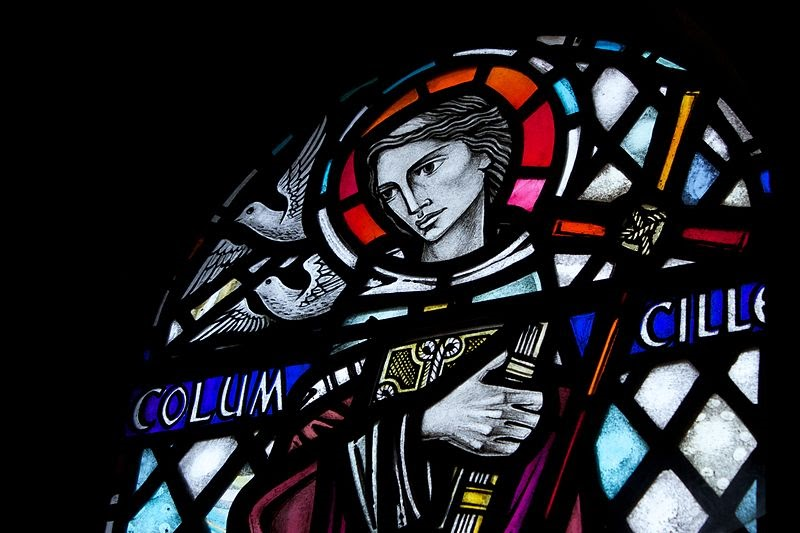
\includegraphics[width=\textwidth]{chapters/img/stained-glass_window.png}
    \caption{St \iai{Colm Cille (Columba)}, 6th-century Irish missionary in Britain, on a stained-glass window at Iona Abbey (Photo by Brian Gratwicke, licensed under CC-BY 2.0)}
    \label{fig:christianity}
\end{wrapfigure}

Christianity\is{Christianity} in Britain is much older than Pope Gregory's\ia{Gregory (Pope)} mission. It was brought there in the context of the Roman Empire\is{Roman Empire} in the 1st and 2nd centuries, and took root among the Celtic-speaking locals especially during the 4th and 5th. Later, there was some tension between the local Christian traditions and the new ones brought in by Gregory's missionaries: for instance, the different traditions didn't agree on the correct date for the festival of Easter.
\end{peoplebox}

    
\noindent The problems of studying the prehistory of English go beyond this, however. It's a commonplace to all historical disciplines that the further you go back in time, the harder it gets (all else being equal). It's not just the language we're a little hazy on: the history of Britain and Europe during this period is also less well understood, and the written sources are highly unreliable. That's why we'll find ourselves relying more on different types of evidence in this chapter. On the historical side, we'll give less weight to people's written accounts of the period, and more weight to the evidence unearthed by archaeologists,\is{archaeology} which over the last thirty years has revolutionized our understanding of the period (see \citealp{Fleming2010}, \citealp{Gerrard2013}, \citealp{Higham2013}, and \citealp{Oosthuizen2019}). On the linguistic side, our main methodology is \textsc{linguistic reconstruction}:\is{reconstruction|(} working backwards from our attested records to infer the most likely properties of unattested linguistic stages and varieties.

Linguistic reconstruction has been described as ``basically the darkest of the dark arts, the only means to conjure up the ghosts of vanished centuries'' (Cola Minis 1952,\ia{Minis, Cola} cited in \citealp[107]{Campbell2013}). The main technique we use for linguistic reconstruction is the \textsc{Comparative Method},\is{Comparative Method} which involves comparing attested languages thought to be related in order to extrapolate back to their common ancestor. This is also the technique we use to establish which languages are related to each other, and how closely: see \citet{Campbell2013} for a clear introduction. Regular sound change,\is{regularity of sound change} as introduced in \sectref{englishtoday-sounds}, plays a crucial role here, and the hypothetical ancestor language reconstructed by means of the Comparative Method\is{Comparative Method} is called a protolanguage. The consensus is that English is a member of the Germanic family, whose common ancestor is called \ili{Proto-Germanic}. These languages in turn are part of a larger family, Indo-European, whose ancestor is \ili{Proto-Indo-European}. The convention is to mark reconstructed forms with an asterisk: so, *\emph{dōn}- is the stem of a Proto-Germanic verb meaning `to do', for example.

We'll look only at a tiny selection of \ili{Proto-Germanic} and \ili{Proto-Indo-European} features in the following sections. If you're hungry for more, \citet{Ringe2017} should be able to satisfy you.\is{reconstruction|)}

\subsection{The \emph{aduentus Saxonum}}\label{prehistory-arrival}\is{migration|(}\is{\emph{aduentus Saxonum}|(}
Pretty much everyone knows that English as spoken in the United States was (and is) a language of immigrants -- though they're usually termed ``settlers'' or ``colonists'' (see Chapters \ref{LModE} and \ref{EModE}).\is{colonialism} It's less well known that English wasn't always spoken in England either. The first speakers of Old English arrived in Britain during the 5th and 6th centuries.\footnote{The term ``Anglo-Saxon'' is often used to describe these speakers, but in this book we'll avoid it, except when referring to other sources. In the modern era it is a term that is more often associated with white supremacists, and has recently been problematized for that reason \citep{RambaranOlm2018,Wilton2020}. It's not a term that writers of Old English used to describe themselves: for this they preferred \emph{englisc}, when they used a term at all. Grouping the Germanic speakers in Britain together as ``Anglo-Saxons'' also implies a static, overarching ethnopolitical unity for which there is no evidence in the historical record \citep{Reynolds1985}, as we'll see in this section.} Before that time, the inhabitants of Britain and Ireland would almost all have been speakers of Celtic varieties (potentially with some British Latin\il{Latin, British} thrown in as well; see \citealp{Schrijver2013} and \citealp{Halsall2013}), as mentioned in \chapref{englishtoday}. Between the first and the fifth centuries CE, most of Britain was part of the Roman Empire.\is{Roman Empire}

The arrival of speakers of Germanic languages in Britain is often referred to as the \emph{aduentus Saxonum}. Sometimes this process is described as an ``invasion'', but the term isn't a very apt one. It implies a large, unified invading army, and a large amount of military conflict. The archaeological\is{archaeology} evidence shows that this wasn't what happened, however. Battles leave material traces -- mass graves, for instance -- and there is very little such evidence. More importantly, the consensus at present is that the arrival of Germanic speakers did not involve the death or displacement of the majority of the indigenous population. Instead, though the scale of migration of Germanic-speaking peoples was relatively small, they were probably able to assume a position of power both politically and culturally \citep[103--105]{Higham2013}. This \textsc{elite dominance} view of the \emph{aduentus Saxonum} is the most widely accepted narrative, but by no means the only one (see \citealp{Fleming2010} and \citealp{Oosthuizen2019}). The relationship between the newcomers and the indigenous speakers of Brythonic Celtic\il{Celtic, Brythonic} has been described in terms of slavery\is{slavery} \citep{Pelteret1995}, but also apartheid \citep{Woolf2007}, and its linguistic implications have been discussed briefly in \sectref{OE-Celtic} above. Emerging approaches to the past, such as palaeobotany, population genetics,\is{genetics} and studies of ancient DNA, have the potential to shed light on this picture. Like other historical witnesses, though, this evidence yields results that can be interpreted in more than one way, and each approach has its own strengths and weaknesses.


\begin{sourcebox}{Evidence from written sources}
There are few written sources describing the \emph{aduentus Saxonum}, and none of the British sources are contemporary. The most famous sources are the writings of \iai{Bede} and the Old English Chronicle, but as Christian\is{Christianity} monks associated with centres of political power the writers of these texts have a clear motive to exaggerate the prowess of the Germanic-speaking military leaders and to play up the dramatic discontinuity of the \emph{aduentus}. Even more problematically, these texts are not really contemporary: they were written hundreds of years after the events that they describe, and are based on sources that are themselves problematic, such as Gildas's\ia{Gildas} \emph{Ruin and Conquest of Britain}, from the sixth century. \iai{Gildas}, who wrote in \ili{Latin}, regarded the incomers as a curse sent by God to punish the indigenous peoples for their deviant ways. Gildas's\ia{Gildas} text is an extended argument (really more of a rant), judging the behaviour of all of Britain's inhabitants according to Roman social norms and trenchantly criticizing them for their -- in his view illegitimate -- military activities \citep{Harland2017}. It is not a narrative history, and neither \iai{Gildas} nor \iai{Bede} can be taken at face value. As a thought experiment, you might like to imagine a future historian's view of the early 21st century if they had to rely solely on Donald Trump's\ia{Trump, Donald} Twitter\is{media} feed, or on the manifesto of your least favourite political party.
\end{sourcebox}


\noindent The extent to which the \emph{aduentus Saxonum} involved military engagement is still disputed. The standard story, dating back to Victorian historians and through them to written sources such as \iai{Bede}'s \emph{Ecclesiastical History}, is that the first Germanic speakers in Britain were mercenaries, invited over from the Continent to help out in turf wars between Celtic-speaking peoples and against raiders from the north and west of the Isles. According to \iai{Gildas}, the thin end of the wedge involved three ships which arrived in Kent in 449 CE. These events were made possible by the weakening of Roman imperial power and the withdrawal of the legions, as well as the subsequent loss of trade connections with continental Europe, in the second half of the fourth century. In an archaeologically-informed\is{archaeology} revisiting of this narrative, \citet[104]{Higham2013} comes to the conclusion that it is broadly plausible, but that there was no mass migration involved. \citet{Fleming2010} takes a different view, arguing that the early Germanic-speaking settlers ``seemed uninterested in and incapable of conquering anybody or anything. They wanted land to farm, and they must have hoped for woods where their swine could forage'' \citeyearpar[40]{Fleming2010}. According to Fleming, migration from Europe was more of a fluctuating stream over centuries than a targeted military strike in a single year, and involved women and children as well as (military and non-military) men. The overall story was one of settlement, acculturation and accommodation. \citet{Oosthuizen2019} suggests that the end of Roman rule in the fifth century involved more continuity than change, with Romano-British administrative structures and rights of property remaining intact. Exactly how much continuity and how much change there was in the period leading up to 600 CE is likely to remain a topic of much debate over the coming years.

\hspace*{-5pt}What evidence about the \emph{aduentus} can we glean from the archaeological record?\is{archaeology} Here it is important to bear in mind that correlations between languages, material culture and genetic\is{genetics} evidence are always fuzzy and full of exceptions: objects, languages, and genes may -- and often do -- diffuse independently of one another. Burial practices are one potential source of evidence. The fourth-century inhabitants of Britain buried their dead intact, but in the fifth century we start to see the rise of cremation, with the ashes of the deceased placed in a pottery urn. This rise has been linked with the arrival of Germanic-speaking newcomers (see \citealp[195--207]{Gerrard2013}). We can also look at what people buried alongside their dead. Different styles of brooches are found in different areas, for instance. Cruciform (cross-shaped) brooches, square-headed brooches, and saucer brooches are found in the south and east of England in the fifth and sixth centuries (\citealp[45--54]{Fleming2010}; \citealp[78--87]{Higham2013}; \citealp{Martin2015}). This archaeological\is{archaeology} evidence maps fairly well onto evidence from place names of Germanic rather than Brythonic Celtic\il{Celtic, Brythonic} or \ili{Latin} origin. Broadly speaking, this evidence also lines up with findings from recent genetic\is{genetics} studies of the present-day British population (e.g. \citealt{Leslie2015}). All these types of evidence show signatures of fifth- and sixth-century influence from the Continent in the south and particularly the east of England.\footnote{We see the reverse influence too: coins and other items that were undoubtedly produced in Britain are found at sites in northern Germany dating from the fourth to sixth centuries \citep{Gruenewald2019,Rau2019}, showing that the North Sea was by no means a one-way street at this time.}

\begin{figure}
        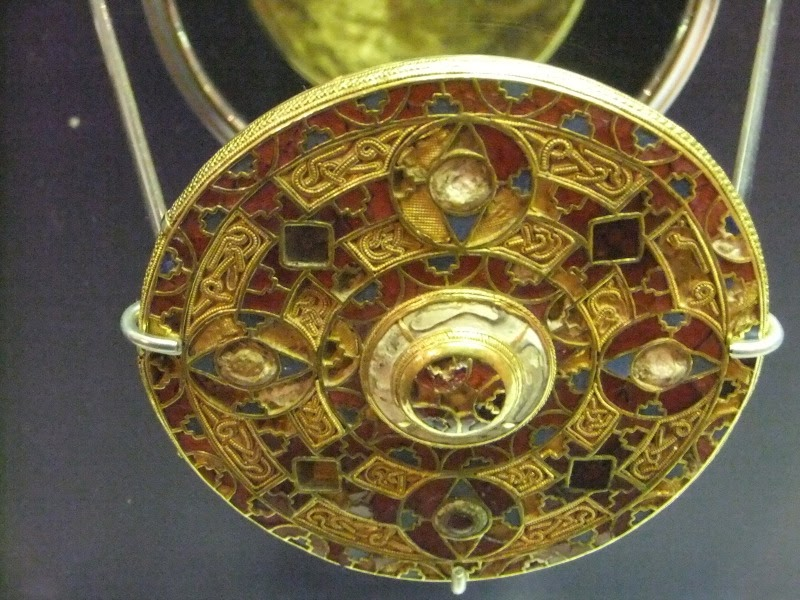
\includegraphics[scale=0.3]{chapters/img/Kingston_brooch.png}
    \caption{The Kingston Brooch, a 7th-century composite brooch found at Kingston Down in Kent (Photo by Rept0n1x, licensed under CC-BY 3.0)}
    \label{fig:kingston_brooch}
\end{figure}

Still, it's important to remember that these practices and features were stunningly diverse. \iai{Bede} famously divided the immigrants into three tribes: Angles, Saxons, and Jutes. Research has provided no support for any such clear division. Cemeteries differed substantially from place to place. The expression of gender identity and gendered norms could differ, for instance.\is{gender studies} Conventionally, men were associated with weaponry and women with jewelry during this period, but in some cemeteries (e.g. West Heslerton in North Yorkshire), men are buried with jewelry, while in others (e.g. Buckland, Dover) women are buried with weapons. Some cemeteries included graves where the deceased was accompanied by tiny pots containing the ashes of pets such as dogs and horses. In others, tree branches were placed in the grave. Saucer-shaped brooches are found more in the south and west of what is now England, while cruciform brooches are more common in the north, but these areas overlapped substantially. There must have been an equal level of linguistic diversity, too, with individuals exploring new ways of constructing their identities in this new and promising environment, just as we see in the present day when different varieties of English and other languages come into contact (as we saw in Chapters \ref{englishtoday} and \ref{LModE} in particular). Unfortunately, the lack of texts means that we'll never know for sure.

All in all, the evidence does not point to any clear ``tribal'' or ethnic groupings for the period before 600: ``distinctive ethnic identities had probably not yet coalesced'' \citep[49]{Fleming2010}. Modern archaeological\is{archaeology} and historical research recognizes that ethnicity is a situational construct: it's not objective or genetic,\is{genetics} but rather is constructed by groups according to their needs in any given situation. These constructed identities, insofar as they existed during this period, must have been complex and multifaceted \citep{Hills2015,Martin2015}. One strand of recent research has made the case that the explanatory value of ethnicity for this period is limited to nonexistent \citep{Harland2017,Harland2019,Oosthuizen2019}.\is{migration|)}

% \begin{figure}
%         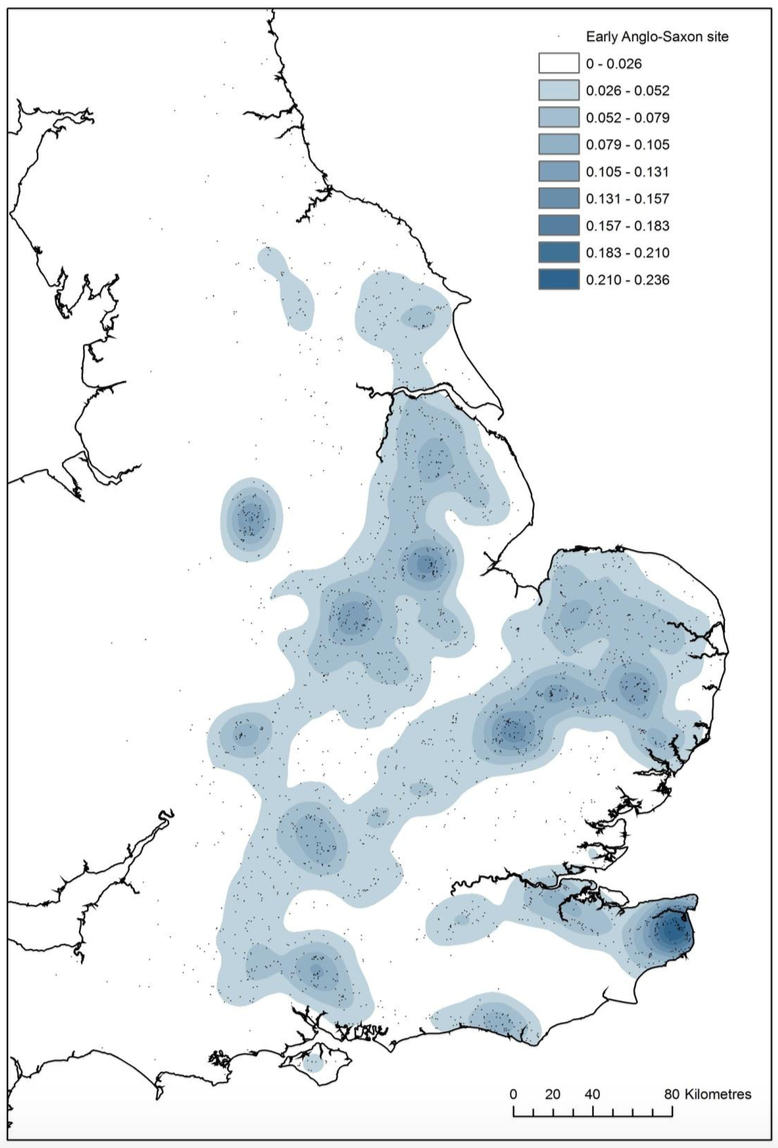
\includegraphics[scale=0.33]{chapters/img/Anglo-Saxon_burial_sites.png}
%     \caption{Density of fifth- and sixth-century Anglo-Saxon burial sites and stray finds of metalwork, from \citet[CCCX]{Martin2011} (Map by Toby F. Martin,\ia{Martin, Toby F.} licensed under CC-BY-NC-ND 2.0)\is{\emph{aduentus Saxonum}|)}}
%     \label{fig:burial-sites}
% \end{figure}

\subsection{The Germanic family}
The peoples who were to become the speakers of Old English migrated\is{migration} from continental Europe. Both the texts and the archaeological\is{archaeology} evidence point us at what is now northern Germany and southern Denmark as their point of origin. As such it's probably not surprising that \emph{Beowulf}, the most famous Old English literary text, is explicitly about the Danes.

We know a few things about the Germanic-speaking peoples of this area and others, but much is lost to the mists of time. Like the pre-Christianization\is{Christianity} Old English speakers, and like many societies of the world until very recently, the Continental Germanic-speaking peoples of Europe pre-600 didn't do much writing. The main contemporary text dealing with these peoples is by Tacitus,\ia{Tacitus, Publius Cornelius} a Roman administrator and politician, and was written around 98 CE. It describes a range of ``tribes'', the \emph{Germani}, who lived in a large area of central and northern Europe, between the northern borders of the Roman Empire\is{Roman Empire} and the North Sea and Baltic coasts. We must treat Tacitus's text with caution, as we know that he himself had never travelled to this area, and all of his information is second- or third-hand. When Tacitus praises the monogamy of the \emph{Germani}, for instance, he's as likely to be making a political point (by contrasting them with what he saw as the immoral practices of his Roman compatriots) as he is to be faithfully reporting the real situation. It's also debatable whether all the groups Tacitus\ia{Tacitus, Publius Cornelius} described as \emph{Germani} were really speakers of Germanic languages.

\begin{figure}[ht]
        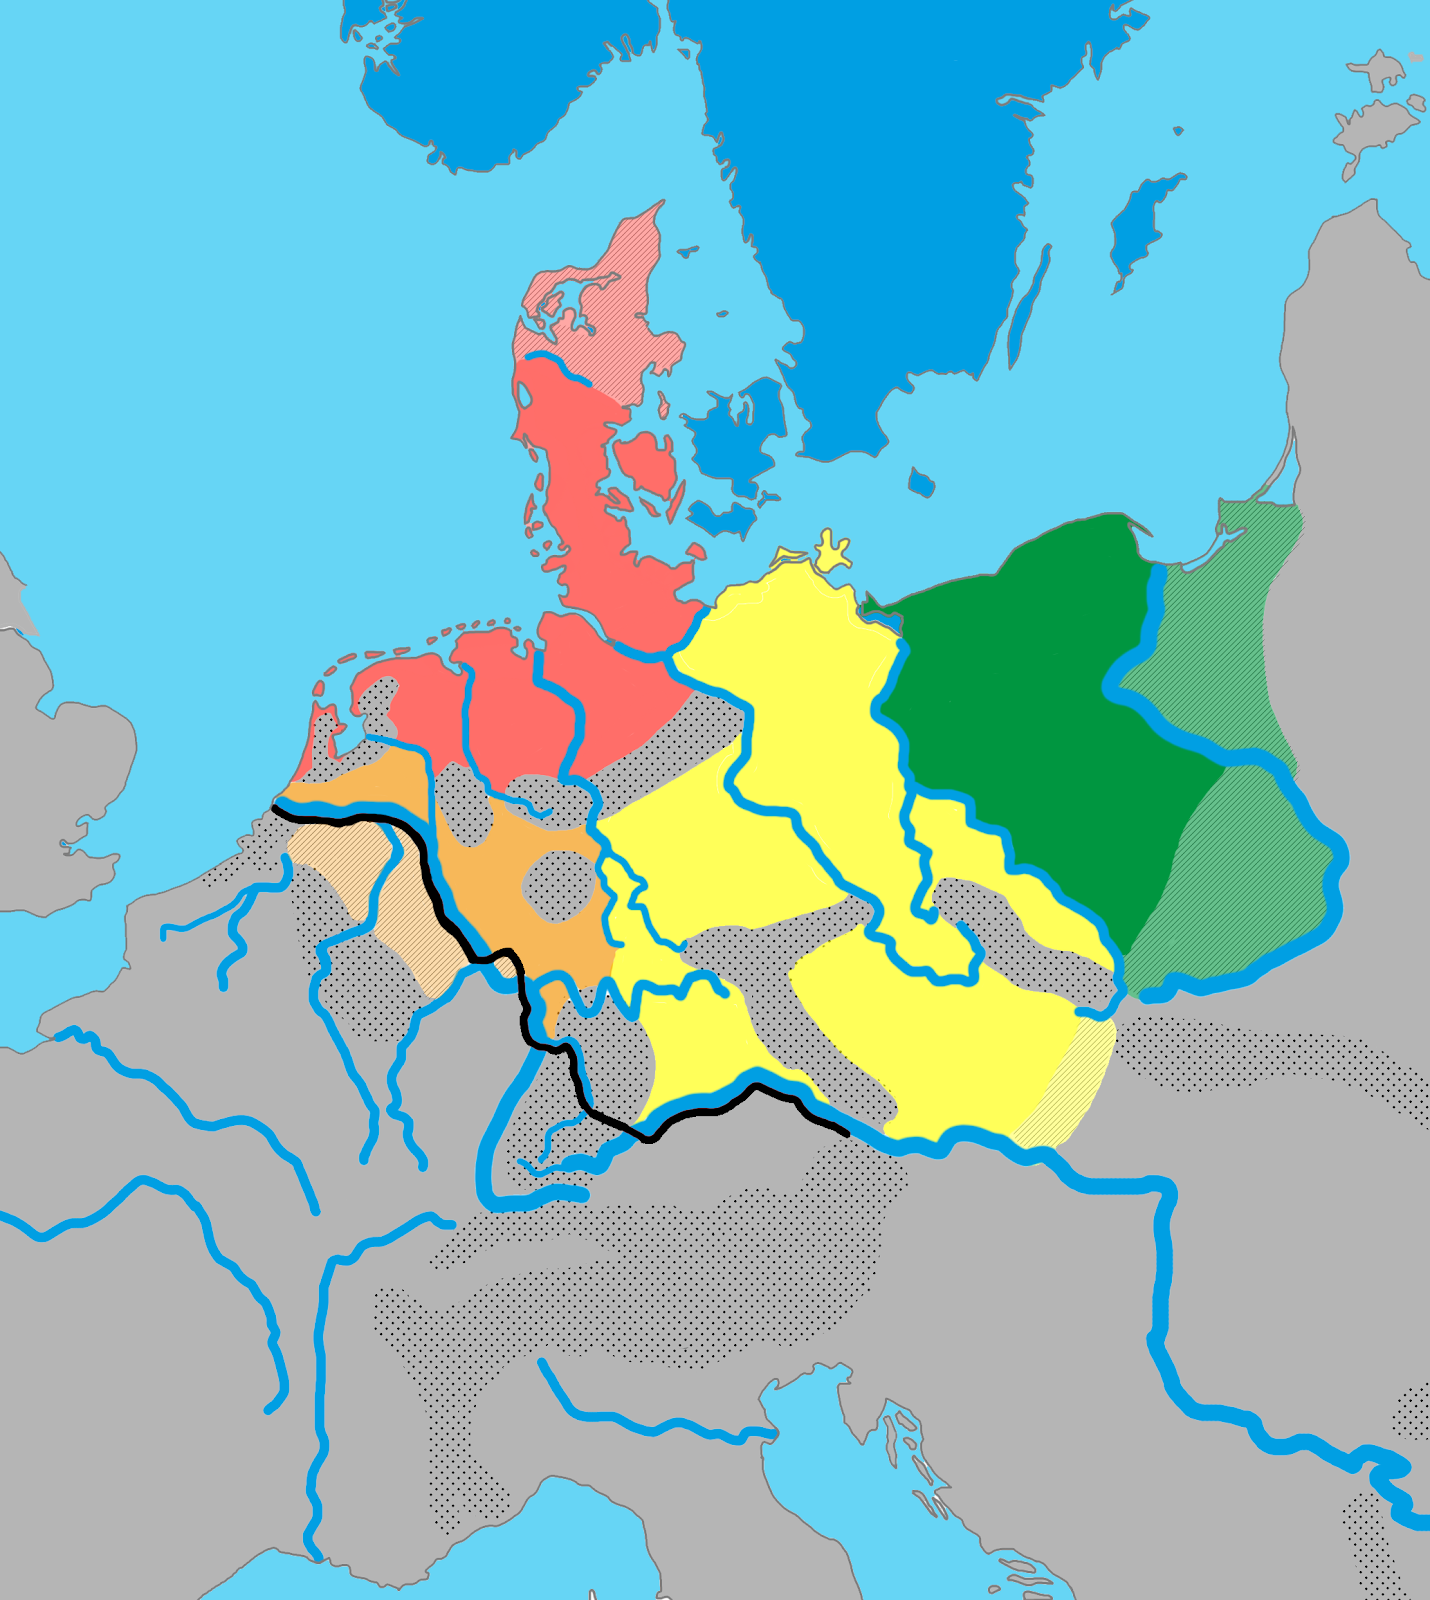
\includegraphics[scale=0.2]{chapters/img/germanic-varieties-tacitus.png}
    \caption{Germanic peoples around 1 CE, following Tacitus.\ia{Tacitus, Publius Cornelius} The black line is the contemporary Roman border. Different colours represent approximate locations of different groups of Germanic speakers. (Map by AKAKIOS, licensed under CC-BY-SA 2.5)}
    \label{fig:Tacitus}
\end{figure}

As usual, the archaeological\is{archaeology} evidence is more tangible, even if it remains silent on many of the most intriguing social details. The peoples living in these areas were skilled wood- and metalworkers, and the organization of their settlements was more complex and sophisticated than the written records imply \citep{Todd2005}, including fortified settlements. Excavations of the settlement at Feddersen Wierde, on the coast of north-western Germany, for instance, show that at its peak as many as fifty families -- each with a separate longhouse -- may have called it their home. Animal husbandry, especially of cattle, played a central economic role. When they fought, these peoples mostly fought on foot, as infantry. Tacitus and other sources mention a wide range of tribal names -- Alamanni, Franks, Goths, Vandals, and more -- but recent research has shown that it is a mistake to view them as fixed political, geographic or ethnic groupings with firm pedigrees. Rather, as far as we can tell, these groupings emerged opportunistically and organically, under individual leaders and in response to the circumstances of the times (see e.g. \citealp{Drinkwater2007} on the Alamanni). Some of the names mentioned by Tacitus,\ia{Tacitus, Publius Cornelius} like \emph{Germani} itself, were never used by the peoples themselves as far as we know, but rather were imposed on them by the Roman world.

We can divide the Germanic languages -- both present and past -- into three groups: East Germanic, North Germanic, and West Germanic. The East Germanic languages are now extinct, and the only language of this group that we know much about is \ili{Gothic}, which is preserved mainly in a 4th-century translation of parts of the Bible. This translation consists mostly of books of the New Testament, and was supervised by a Gothic bishop with the adorable name of \iai{Wulfila} (`little wolf'): see the text samples at the end of this chapter. The Goths were major players in the politics of Europe in the first millennium, especially during the twilight of the Roman Empire\is{Roman Empire} (see \citealp{Heather1996}). Because of the age of its attestation, Gothic is the closest of the well-attested early Germanic languages to Proto-Germanic. Still, \ili{Gothic} displays several linguistic features that set it apart from all other Germanic languages, and the other two branches -- North and West Germanic -- are probably more closely related \citep{Kuhn1955}.

\begin{figure}\small
    \qtreecentertrue \Tree [.Proto-Germanic [.Northwest~Germanic [.West~Germanic [.Anglo-Frisian [.Old~English English ] [.Old~Frisian Frisian ]] [.Old~Saxon Low~German ] … ] [.North~Germanic Danish … ]] [.East~Germanic Gothic ]]
    \caption{Partial Germanic family tree}
    \label{fig:partial-germanic-family-tree}
\end{figure}

\largerpage
The North Germanic languages survive robustly to this day, mostly in Scandinavia: varieties of \ili{Danish}, \ili{Faroese}, \ili{Icelandic}, \ili{Norwegian}, and \ili{Swedish} all belong to this group, as did the \ili{Norse} spoken by the Scandinavians who settled in Britain during the 9th to 11th centuries (see \sectref{OE-Scandinavian}). The West Germanic branch includes \ili{Afrikaans}, \ili{Dutch}, \ili{Frisian}, \ili{German}, \ili{Yiddish}, and English. The internal structure of the West Germanic branch is still debated (see \citealp{Stiles2013} for a recent overview), though is not too important for our purposes. Within West Germanic, English's closest relative is \ili{Frisian}, a collection of related varieties currently spoken along the North Sea coast of the Netherlands, Germany and Denmark, and endangered to some extent.


\begin{varietybox}{English as a cuckoo in the nest}
The majority view is that English is a West Germanic language, but not everyone shares this view. Recently it has been proposed that modern English is a North Germanic language: see \citet{BechWalkden2016} for a sceptical evaluation. Another view is that, due to its extensive history of language contact, English is now a language without any relatives whatsoever, a creole\is{creoles} -- which arose through contact with either Norman French\il{French, Norman} \citep{BaileyMaroldt1977} or \ili{Norse} \citep{Poussa1982}. \citet{Gorlach1986} presents arguments against both claims. No one disputes that Old English was a West Germanic language, however.
\end{varietybox}



\noindent There are no texts longer than a few sentences from either North or West Germanic from pre-600: all we have are brief inscriptions (see \sectref{prehistory-sounds}). The closest language to Old English that is attested in the first millennium CE is Old Saxon,\il{Saxon, Old} a West Germanic language probably spoken between the rivers Elbe and Weser. We have Old Saxon texts from the 9th century onwards, and there's a text sample at the end of this chapter. Modern-day dialects of northern Germany are the living descendants of Old Saxon.\il{Saxon, Old} \citet{Robinson1992} provides more information on the other early Germanic languages, Old English's closest relatives.

\subsection{Indo-European and the Indo-Europeans}
The Germanic languages descend from Proto-Germanic, which in turn is part of a larger family, Indo-European. The establishment of this family was one of the major achievements of nineteenth-century comparative linguistics (see \citealp{Clackson2007} for an accessible overview), and a family tree can be found in Figure \ref{fig:partial-IE-family-tree}.

\begin{figure}\scriptsize
    \qtreecentertrue \Tree [.Proto-Indo-European [.Anatolian … ] [[ [.Balto-Slavic [.Baltic … ] [.Slavic … ]] [.Germanic … ] [ Armenian [.Hellenic Greek ]] [.Indo-Iranian … ] [.Italo-Celtic [.Celtic … ] [.Italic … ] ]] Tocharian ] ]
    \caption{Partial Indo-European family tree 
(loosely based on \citealp[90]{RingeWarnowTaylor2002}, their Figure 8)}
    \label{fig:partial-IE-family-tree}
\end{figure}

\noindent Almost all the languages of Europe are demonstrably part of this family. (\ili{Basque}, \ili{Estonian}, \ili{Finnish}, and \ili{Hungarian} are notable exceptions.) This includes all the languages that had a major influence on English before the colonial period: \ili{Latin} (part of the Italic branch), \ili{French} (ultimately descended from \ili{Latin}), the Celtic languages (which form their own branch), \ili{Greek}, and of course \ili{Norse}, as we saw in Chapters \ref{EModE}–\ref{OE}. The family also has several members which are further afield, and perhaps more surprising: \ili{Armenian}, for instance, and the \ili{Indo-Iranian} languages spoken in central and southern Asia, including the ancient language \ili{Sanskrit}.

All Indo-European languages ultimately descend from a single ancestor, \ili{Proto-Indo-European}. The speakers of Proto-Indo-European are even more of a mystery than the speakers of \ili{Proto-Germanic}. No texts go back that far, so we are entirely dependent on reconstruction\is{reconstruction} and on the archaeological\is{archaeology} record to tell us about the people who spoke the language (though evidence from ancient genetic\is{genetics} material is starting to play a role as well -- see \citealt{Haak2015}). The usual story (starting with \citealp{Gimbutas1970}) is that \ili{Proto-Indo-European} was spoken between 4,000 and roughly 2,000 BCE, and originated in the Pontic-Caspian steppes, in present-day Ukraine and southern Russia: this is labelled the ``Kurgan hypothesis'' or ``steppe hypothesis''. Synthesizing the linguistic and archaeological\is{archaeology} evidence, \citet{Anthony2007} makes the case that the domestication of the horse and the invention of the wheel, along with new modes of social and political organization, contributed to the spread of the Indo-Europeans and their language across Europe and beyond.\footnote{For a recent overview that also takes ancient DNA\is{genetics} evidence into account, see \citet{Anthony2019}.} As these newcomers and their culture fanned out across Europe, the language diversified into varieties that were mutually unintelligible, through exactly the processes of linguistic change that we've been exploring throughout this book (see e.g. \chapref{englishtoday} on homogeneity and heterogeneity).


\begin{varietybox}{Before Proto-Indo-European?}
\ili{Proto-Indo-European} cannot have been spoken before the 7th millennium BCE at the very earliest. However, research on the evolution of the human capacity for language (see \citealp{Fitch2010}) has demonstrated that this capacity has been around in its modern form since the 50th millennium BCE at the very latest. This book therefore only covers at most 10\% of the history of English and its predecessors, and if we disregard the present chapter it's more like 1–2\%. Can we go any further back? The short answer is ``not really''. Some linguists have proposed more distant relationships between Indo-European and other language families such as Afro-Asiatic (including \ili{Arabic} and \ili{Hebrew}), Uralic (including \ili{Finnish} and \ili{Hungarian}), and Kartvelian (including languages of the Caucasus such as \ili{Georgian}). However, the consensus in linguistics is that the time depth is too great, and the evidence too weak, to be anything other than suggestive: the usual tools such as the Comparative Method\is{Comparative Method} yield inconclusive results \citep{CampbellPoser2008}. Thus, with \ili{Proto-Indo-European} we reach the earliest portion of the history of English that is accessible by normal means, and the clouded realm of linguistic prehistory looms before us.
\end{varietybox}


\section{Sounds}\label{prehistory-sounds}
\subsection{Old English and Frisian vowels}\label{prehistory-vowels}\is{vowels|(}
One major feature setting Old English (and also Old Frisian)\il{Frisian, Old} apart from the other Germanic languages was a series of changes to their vowels, which have the picturesque name of ``Anglo-Frisian Brightening''.\is{Anglo-Frisian Brightening} West Germanic long [ɑː] became [æː], and a little later short [a] became [æ] as well. This gives us words like Old English \emph{dæġ} `day', \emph{mæġ} `may' and \emph{strǣt} `street', compared to (for instance) Old Saxon\il{Saxon, Old} \emph{dag} `day', \emph{mag} `may' and \emph{strāt-} `street', which did not undergo the change.

Nasalized [ɑ̃], and [ɑ] followed by /n/ or /m/, were unaffected by Anglo-Frisian Brightening,\is{Anglo-Frisian Brightening} however. These sounds later raised to [õ] and [o] in both Old English and Old Frisian,\il{Frisian, Old} giving us words like Old English and Old Frisian \emph{mon} `man' whereas the Old Saxon cognate \emph{man} remained unchanged. The same happened to the long vowels [ɑ̃ː] and [ɑː], yielding for instance Old English \emph{mōn-} `moon' rather than Old Saxon\il{Saxon, Old} \emph{mān-} `moon'. It is actually not uncommon for nasal consonants,\is{consonants} such as /n/ and /m/, to raise the preceding vowel at various points in time in the history of the English language. Thus, we can observe e.g. the so-called \emph{pin-pen} merger\is{merger} in some dialects of American English\il{English, American}, but there are more raising processes taking place before nasals in Present Day English.

Old Frisian\il{Frisian, Old} later raised [æ] to [ɛ] and [æː] to [ɛː], giving us (for instance) \emph{dei} `day' and \emph{strēt-} `street'. Thus, the presence of the letter <æ> is a sure-fire way to tell that you're dealing with an Old English text! However, there is variation between and within dialects with regard to the sound changes discussed in this section \citep[167--170]{RingeTaylor2014}. This variation probably reflects the fact that these sound changes were still in progress at the time of the arrival of Germanic speakers in Britain \citep{Toon1992}, as this sort of variability is exactly what we see in present-day changes in progress (see \chapref{englishtoday}).\is{vowels|)}

\subsection{Runes and runic inscriptions}\label{prehistory-runes}\is{runes|(}
Before 600 CE, we don't find Germanic languages written in the Latin alphabet.\is{orthography|(} Rather, the few surviving Germanic writings from this period (with the exception of some texts in \ili{Gothic}) use a different writing system: the runic alphabet.

\begin{table}
    \caption{The runic alphabet (Older Futhark), from \citet[18]{Findell2014}}\label{runic-alphabet}
  \begin{tabular}{lll}
\lsptoprule
    Rune & Transliteration & Sound value \\ \midrule
    \textarc{f} & f & [f] \\
    \textarc{u} & u & [u] \\
    \textarc{\th} & þ & [θ] \\
    \textarc{a} & a & [a] \\
    \textarc{r} & r & [r] \\
    \textarc{k} & k & [k] \\
    \textarc{g} & g & [ɡ] \\
    \textarc{w} & w & [w] \\
    \textarc{h} & h & [h] \\
    \textarc{n} & n & [n] \\
    \textarc{i} & i & [i] \\
    \textarc{j} & j & [j] \\
    \textarc{p} & p & [p] \\
    \textarc{I} & ï & [i] (?) \\
    \textarc{R} & z & [z] \\
    \textarc{s} & s & [s] \\
    \textarc{t} & t & [t] \\
    \textarc{b} & b & [b] \\
    \textarc{e} & e & [e] \\
    \textarc{m} & m & [m] \\
    \textarc{l} & l & [l] \\
    \textarc{\ng} & ŋ & [ŋ], [ŋɡ], [iŋɡ] \\
    \textarc{d} & d & [d] \\
    \textarc{o} & o & [o] \\
    \lspbottomrule
  \end{tabular}
\end{table}

\noindent We have runic inscriptions from all across the Germanic world, from the 2nd century CE onwards. You'll notice that, unlike the \ili{Latin} alphabet, the runic characters consist entirely of straight lines. This is because they were designed to be carved into hard surfaces, not scribed\is{scribes} with ink: in fact, the English verb \textit{to write} is descended directly from a Proto-Germanic verb meaning `to carve'.


\begin{sourcebox}{Futhark or Futhorc?}
The original twenty-four-character runic alphabet is known as the \textsc{futhark}, after its first six characters -- much like the QWERTY keyboard, the usual layout for keyboards in the \ili{Latin} alphabet. It is sometimes known as the Older Futhark to distinguish it from its descendant the Younger Futhark, which developed in Scandinavia from the 7th century onwards. In Britain, at around the same time, the \textsc{futhorc}, a slightly expanded set of runes, came into use. The futhorc better reflected the new vowel\is{vowels} system of Old English (see \sectref{prehistory-vowels} above): the rune <\textara{\ae}> came to represent [æ], and the new runes <\textara{a}> for [ɑ], <\textara{o}> for [ɑ̃] (later [õ]), and <\textara{\oe}> for [œ] are found for the first time.
\end{sourcebox}


\noindent The runic alphabet in fact tells us a few interesting things about the phonological system of the early Germanic languages. For instance, the rune <\textarc{\th}>, called \glossterm{gl-thorn}{thorn},\is{thorn} represents the \glossterm{gl-phoneme}{phoneme} /θ/. The \ili{Latin} alphabet had no convenient way to represent this sound -- unsurprisingly, as the Latin language itself didn't have the sound. The thorn rune was so useful that scribes\is{scribes} of Old English kept using it even when they were otherwise writing in the \ili{Latin} alphabet, and that's where the Old English letter <þ> comes from. Thorn\is{thorn} was lost in Middle English, and nowadays we write this sound as <th>, but that's a poor substitute (try pronouncing [t] and [h] together and you'll see that it's nothing like [θ]).

\begin{figure}
        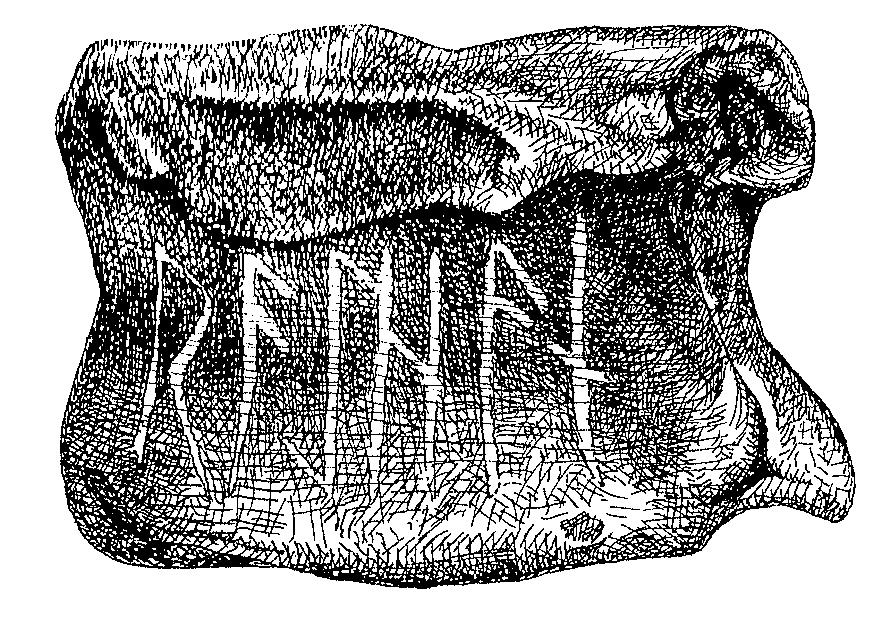
\includegraphics[scale=0.5]{chapters/img/runic-inscription.jpg}
    \caption{The anklebone of a roe deer, found in Caistor-by-Norwich and dated to the 5th century. This is the earliest runic inscription yet found in England. The word written here means `roe'. Try transliterating it yourself!}
    \label{fig:anklebone_runic_inscription}
\end{figure}


\begin{sourcebox}{Bluetooth}
\begin{wrapfigure}{r}{0.2\textwidth}
        
\includegraphics[scale=0.08]{chapters/img/393px-Bluetooth.png}
    \caption{The Bluetooth logo}
    \label{fig:bluetooth}
\end{wrapfigure}
The logo of the wireless technology\is{technology} standard Bluetooth (Figure \ref{fig:bluetooth}) is a rune! In fact, it's two runes used together: <\textarn{h}> and <\textarn{b}>, which in the Younger Futhark stand for /h/ and /b/ respectively. These are the initials of Harald Bluetooth,\ia{Bluetooth, Harald} the tenth-century Danish king who the technology is named after. When two runes are written together like this, the result is called a \textsc{bind rune}.\is{orthography|)}\is{runes|)}
\end{sourcebox}


\subsection{The First Sound Shift}\is{First Sound Shift|(}
We've\is{consonants|(} just seen that the early Germanic languages had the \glossterm{gl-phoneme}{phoneme} /θ/, but that \ili{Latin} -- another Indo-European language -- didn't. What happened here? Does Latin better reflect the inherited \ili{Proto-Indo-European} situation, or does Germanic?

Using the Comparative Method\is{Comparative Method} it's possible to establish that it's Germanic that's the innovator. In fact, the change that Proto-Germanic underwent, some time after 500 BCE, is probably the single most important feature setting the Germanic languages apart from all the other Indo-European languages. This makes it important evidence that the Germanic languages belong together as a group. The change is known as the First Sound Shift, or as Grimm's Law, because it is associated with the 19th-century linguist and mythologist Jacob Grimm\ia{Grimm, Jacob} (part of the famous German ``Brothers Grimm'' duo, along with his brother Wilhelm).\ia{Grimm, Wilhelm} In fact, the much less famous Danish linguist Rasmus Rask\ia{Rask, Rasmus} had got there first, in the year 1818. In any case, the First Sound Shift is the second of the two famous sound changes mentioned in \chapref{englishtoday} (the other being the Great Vowel Shift\is{vowels}\is{Great Vowel Shift} discussed in \sectref{EModE-GVS}).

What Rask\ia{Rask, Rasmus} and Grimm\ia{Grimm, Jacob} noticed was that there were systematic correspondences between certain consonants in the Germanic languages and their counterparts in the other Indo-European languages. For example, where we find a /p/ in other Indo-European languages, we often find a /f/ in Germanic languages, as shown in Table \ref{tab:IE-p_and-Ger-f}.

\begin{table}
        \begin{tabular}{l llll ll}
        \lsptoprule
    Meaning & \ili{Latin} & \ili{Greek} & \ili{Sanskrit} & \ili{Gothic} & Old English & Old Saxon\il{Saxon, Old}  \\
    \midrule
    `foot' & \textbf{p}ed- & \textbf{p}od- & \textbf{p}ā́d- & \textbf{f}ōt- & \textbf{f}ōt & \textbf{f}ōt \\
    `fish' & \textbf{p}isc- &&& \textbf{f}isk- & \textbf{f}isċ & \textbf{f}isk \\
    `five' && \textbf{p}énte & \textbf{p}áñca & \textbf{f}imf & \textbf{f}īf & \textbf{f}īf\\
    \lspbottomrule
\end{tabular}
    \caption{Indo-European /p/ \& Germanic /f/ (based on \citealp[114]{Ringe2017})}
    \label{tab:IE-p_and-Ger-f}
\end{table}

\noindent The full set of changes that make up the First Sound Shift is given in Table \ref{tab:first_Sound_Shift}. Similar corresponding sets of examples can be found for each of these changes. For instance, \ili{Sanskrit} \emph{bhr{a^^^^0304^^^^0301}tṛ} `brother', which starts with a voiced aspirated /bʰ/ and contains a voiceless /t/, corresponds to \ili{Gothic} \emph{brōþar} and Old English \emph{brōþor}, which start with a voiced unaspirated /b/ and contain a voiceless fricative /θ/.

\begin{table}
        \begin{tabular}{llll}
        \lsptoprule
     & \textbf{Labial} & \textbf{Coronal} & \textbf{Velar} \\
     \midrule
    \textbf{voiceless stops > fricatives} & p > f & t > θ & k > x \\
    \textbf{voiced stops > voiceless stops} & b > p & d > t & ɡ > k \\
    \textbf{voiced aspirated stops > plain voiced stops} & bʰ > b & dʰ > d & ɡʰ > ɡ \\
    \midrule
\end{tabular}
    \caption{The First Sound Shift (after \citealp[42]{Campbell2013})}
    \label{tab:first_Sound_Shift}
\end{table}

\noindent The First Sound Shift is a regular sound change\is{regularity of sound change} with far-reaching consequences, and is one of the most striking and characteristic features of the Germanic languages.\footnote{For more detail on the First Sound Shift, see \citet[§3.2.4]{Ringe2017} and \citet[§6.4--§6.7]{Fulk2018}.} You may like to think about whether the First Sound Shift is also a chain shift,\is{chain shifts} in the sense that was discussed in \sectref{NC-shifts} for the Northern Cities Shift\is{Northern Cities Shift} and in \sectref{EModE-GVS} for the Great Vowel Shift.\is{vowels}\is{Great Vowel Shift}


\begin{peoplebox}{Making linguistic history: Rask, Grimm, and Verner}
The version of the First Sound Shift given in Table \ref{tab:first_Sound_Shift} is almost exceptionless, but not quite: for instance, \ili{Sanskrit} \emph{pitṛ́} `father' contains a /t/ that seems to correspond to a /d/ in \ili{Gothic} \emph{fadar} and Old English \emph{fæder}, rather than the expected /θ/. Rask\ia{Rask, Rasmus} and Grimm\ia{Grimm, Jacob} were working in an era before the regularity of sound change\is{regularity of sound change} was postulated, and were aware of some exceptions to their generalization. It wasn't until 1875 that another Danish linguist, Karl Verner,\ia{Verner, Karl} was able to show that these exceptions were themselves governed by a robust rule. In fact, Verner's discovery played an important role in the establishment of the regularity of sound change as a guiding principle in historical linguistics during the 19th century. See \citet[140--142]{Campbell2013} for the details of ``Verner's Law'', and \citet[132--135]{Lass1997} for a critical assessment of Verner and regular sound change. (Search for Verner's Law and the Studies in Germanic Philology on YouTube if you'd like to watch a highly amusing film on these linguistic discoveries.)\is{consonants|)}\is{First Sound Shift|)}
\end{peoplebox}


\subsection{The Germanic stress shift}\label{prehistory-stress}\is{stress shift|(}
Another change that divides the Germanic languages from many of their more distant Indo-European family members has to do with the positioning of lexical stress within a word. We can reconstruct\is{reconstruction} earlier Indo-European, before Germanic branched off, as having a stress system that was lexically variable (similarly to Present Day English: compare \emph{photo}, \emph{photography}, and \emph{photographic}, with the stress on the first, second, and third syllables respectively). This system was present in Vedic \ili{Sanskrit}, for instance. Different words have their primary stress on different syllables: for example, \emph{bhr{a^^^^0304^^^^0301}tṛ} `brother' is stressed on the first syllable, while \emph{pitṛ́} `father' is stressed on the second (a syllabic /r/).\is{/r/} In \ili{Proto-Germanic}, by contrast, the stress became fixed on the first lexical \glossterm{gl-morpheme}{morpheme} of the word, which usually corresponded to the first syllable of the word. Thus, in the early Germanic languages, all words have initial stress, with the exception of some unstressed verbal prefixes\is{affixes} such as Old English \emph{ġe}-.\footnote{Similar stress-fixation changes affected other branches of the Indo-European language families at different stages of their historical paths.}

Fixing the stress on the first syllable of the word had various consequences. For one thing, a tradition of \textsc{alliterative poetry}\is{poetry}\is{alliteration} developed in Germanic, and some of these poems are preserved in many of the early Germanic languages -- including Old English, Old Saxon,\il{Saxon, Old} Old High German\il{German, Old High} and Old \ili{Norse}. The most famous example of Old English alliterative\is{alliteration} verse is \emph{Beowulf}, but there is much more.\is{poetry}

Alliterative verse differs from rhyming verse in that what's important is not the end of the syllable (as in rhyming verse, e.g. \emph{p\textbf{ill}} vs. \emph{f\textbf{ill}}) but rather the first consonant\is{consonants} of the first syllable of the word. This sort of verse survives into Middle English, and the first line of William Langland's\ia{Langland, William} poem\is{poetry} \emph{Piers Plowman} is an accessible example: \emph{In a \textbf{s}omer \textbf{s}eson, whan \textbf{s}oft was the \textbf{s}onne} `In summer, when the sun was soft'. Here the alliteration is on the phoneme /s/. Clearly, word-initial stress and alliterative verse are a match made in heaven, and linguistically it's no surprise that in Present Day English, with its more complex stress system, alliterative verse is not the dominant tradition any more. If you want to learn more about Old English alliterative\is{alliteration} poetry,\is{poetry} \citet[unit 5]{McCullyHilles2005} is a great introduction.

The fixation of stress on the initial syllable also may have had consequences for the morphology of the Germanic languages. \ili{Proto-Germanic} had a variety of vowels\is{vowels} in unstressed syllables, similar to (early) Old English (\chapref{OE}), and these can still be seen in the \ili{Gothic} Bible and the earliest runic inscriptions, as well as to some extent in Old English and Old Saxon\il{Saxon, Old} texts. A common tendency across all the Germanic languages was to lose these vowels\is{vowels} entirely, or for them to lose their distinctiveness and merge\is{merger} together as schwa /ə/.\is{vowel reduction} These unstressed syllables, however, often carried important morphological distinctions, especially when word-final: different cases,\is{case} for instance, or different person and number forms of the verb. The only difference between the Old English past tense plural\is{plurals} forms of the verb `to help', \emph{hulpon} (indicative \glossterm{gl-mood}{mood}) and \emph{hulpen} (subjunctive mood),\is{subjunctive} for example, is the vowel in the unstressed syllable: /o/ in the indicative and /e/ in the subjunctive.\is{subjunctive} When the distinctive vowel\is{vowels} quality was lost, the morphological distinction it conveyed was often also lost. Thus, a change that dates back to the birth of the Germanic family was still making itself felt many centuries later. Note, though, that the fixation of stress can't by itself explain why some Germanic languages (like English and \ili{Afrikaans}) ended up losing almost all their morphological endings while others (like \ili{Icelandic} and \ili{German}) were much more conservative.\footnote{There are also other languages where the stress is fixed on the first syllable, such as \ili{Finnish}, which show no signs of vowel\is{vowels} reductions\is{vowel reduction} in unstressed syllables, again suggesting that the fixation of stress isn't the whole story.} For that, a different story is needed: see \sectref{OE-case-loss}.

Yet another consequence of fixing the stress was related to the fate of ablaut.\is{ablaut} More on this in \sectref{prehistory-strong}.\is{stress shift|)}

\section{Morphology}
\subsection{The Germanic weak past tense}\label{prehistory-weakpast}\is{weak verbs|(}
Alongside the First Sound Shift\is{First Sound Shift} and Germanic stress shift,\is{stress shift} a third major change characterizing the Germanic languages but not other Indo-European relatives was the development of a new type of past tense for weak verbs.

\begin{table}
        \begin{tabularx}{\textwidth}{XXl}
    \lsptoprule
    Language & Infinitive & Past (3rd Singular)  \\
    \midrule
    English & play & playe\textbf{d} \\
    \ilit{Danish} & lege & lege\textbf{d}e \\
    \ilit{Dutch} & spelen & speel\textbf{d}e \\
    \ilit{Faroese} & spæla & spæl\textbf{d}i \\
    \ilit{German} & spielen & spiel\textbf{t}e \\
    \ilit{Norwegian} & leke & lek\textbf{t}e \\
    \lspbottomrule
    \end{tabularx}
    \caption{Forms of the past tense of `play' in present-day Germanic languages}
    \label{tab:past_of_play}
\end{table}

\noindent In all of these present-day Germanic languages, and in all the early Germanic languages as well, the regular past tense is formed using a suffix\is{affixes} containing some sort of coronal consonant\is{consonants} -- usually /d/.\footnote{See \sectref{ME-verbs} if you need a reminder of what weak, strong,\is{strong verbs} regular, and irregular\is{irregularities} mean.} But this type of past tense formation is not found elsewhere in the Indo-European family.\footnote{This is a bit of a simplification. Some Iranian languages -- also belonging to Indo-European -- have undergone a very similar development independently. See \citet{Kuemmel2020}.} How did it arise?

As usual with changes that predate the textual record, there are different theories, and we have to decide which is the most plausible. Here we'll briefly illustrate the dominant contender (as summarized in \citealp[191--192]{Ringe2017}), which is that the Germanic weak past in /d/ arose when a sequence consisting of a non-finite verb form and a past tense form of the verb *\emph{dōną} `to do' was reinterpreted as a single word. Basically, two originally independent words got stuck together. Thus, in essence, a form like \emph{played} originated as something like \emph{play did}. This sort of happening is well known in the literature on \glossterm{gl-grammaticalization}{grammaticalization}\is{grammaticalization} \citep{HopperTraugott2003}, where it's usually known as \glossterm{gl-univerbation}{univerbation}. See also the discussion of the Modern English semi-modals\is{modals} in \sectref{LME-semimodals}.

This theory receives direct support from a set of plural\is{plurals} forms in \ili{Gothic}. In this language, the past tense of weak verbs in the plural ends in -\emph{dēdun}, e.g. \emph{nasi\textbf{dēdun}} `they saved/healed', \emph{sōki\textbf{dēdun}} `they sought, looked for'. This reflects exactly the reconstructed\is{reconstruction} \ili{Proto-Germanic} past tense of the verb *\emph{dōną}, which is *\emph{dēdun} in the third person plural.\footnote{Note that the /d/ at the end of the form \emph{*dēdun} is part of the stem, not part of the ending. If it were part of the ending, the theory would be circular, as it would require there to have already been a weak past in /d/ in \ili{Proto-Germanic}, and so its origin would remain unexplained.}\is{plurals} These forms are the only place in Germanic where the assumed historical development is reflected so precisely, and indicate that the verb *\emph{dōną} has to be at least part of the story.

We can't be sure that this is what happened in the prehistory of Germanic. But it does fit with what we know about common pathways of grammatical change, without needing to wave a magic wand and propose a historical development that has no parallel elsewhere. See \citet[191--192]{Ringe2017} for a much more detailed version of the story. This sort of evidence might not stand up in a court of law, but it's good linguistic detective work nonetheless.\is{weak verbs|)}

\subsection{The Germanic strong verbs}\label{prehistory-strong}\is{strong verbs|(}\is{ablaut|(}
Alongside the weak verbs,\is{weak verbs} the strong verbs constituted the other big group of verbs in early Germanic. As we've seen in \sectref{OE-morphology},\footnote{And also in \chapref{ME} for Middle English: \sectref{ME-verbs}.} the endings on strong verbs in Old English were very similar to those of weak verbs, but they differed in how they formed their past tense: where the weak verbs\is{weak verbs} added an ending containing a /d/, the strong verbs changed the vowel\is{vowels} in the stem.

For Present Day English, and to a certain extent for Middle and Old English, the dominant approach to the vowel alternations in the strong verbs is simply to treat them as irregular\is{irregularities} and lexically listed. In other words, for each strong verb, the language user simply has to memorize the relevant past tense forms in their entirety \citep{Pinker1999}. However, things weren't always like this. The further we go back in time, the more we find that the strong verbs follow a neat, orderly system that actually makes sense.

Table \ref{tab:OE-strong-verbs} gives some illustrative forms for the first three classes of strong verbs in Old English (there are seven in total; we'll leave aside classes IV--VII). The column ``1st past'' gives the vowel\is{vowels} used in the first and third persons singular of the past tense; ``2nd past'' gives the vowel used elsewhere in the past tense.

\begin{table}
    \begin{tabularx}{\textwidth}{XXXl}
        \lsptoprule
    \textbf{Class} & \textbf{Sample verb} & \textbf{1st past}  & \textbf{2nd past} \\
    \midrule
    I & \emph{dr\textbf{ī}fan} `to drive' & \emph{dr\textbf{ā}f} & \emph{dr\textbf{i}fon} \\
    II & \emph{cr\textbf{ēo}pan} `to creep' & \emph{cr\textbf{ēa}p} & \emph{cr\textbf{u}pon} \\
    III & \emph{h\textbf{e}lpan} `to help' & \emph{h\textbf{ea}lp} & \emph{h\textbf{u}lpon} \\
    \lspbottomrule
    \end{tabularx}
    \caption{Strong verb classes in Old English}
    \label{tab:OE-strong-verbs}
\end{table}

\noindent Reducing this to its essentials gives us the vowel\is{vowels} system in Table \ref{tab:OE-strong-verbs-vowels}.

\begin{table}
    \begin{tabularx}{\textwidth}{XXXl}
        \lsptoprule
    \textbf{Class} & \textbf{Present} & \textbf{1st past} & \textbf{2nd past}\\
    \midrule
    I & \emph{\textbf{ī}} & \emph{\textbf{ā}} & \emph{\textbf{i}} \\
    II & \emph{\textbf{ēo}} & \emph{\textbf{ēa}} & \emph{\textbf{u}} \\
    III & \emph{\textbf{e}} & \emph{\textbf{ea}} & \emph{\textbf{u}} \\
    \lspbottomrule
    \end{tabularx}
    \caption{Vowels in strong verbs in Old English}
    \label{tab:OE-strong-verbs-vowels}
\end{table}

\noindent Things are even more transparent if we consider the Proto-Germanic ancestors of these vowels:\is{vowels} see Table \ref{tab:PGmc-strong-verbs-stems}.

\begin{table}
    \begin{tabularx}{\textwidth}{XXXl}
        \midrule
    \textbf{Class} & \textbf{Present} & \textbf{1st past} & \textbf{2nd past}\\
    \midrule
    I & \emph{\textbf{ei > ī}} & \emph{\textbf{ai}} & \emph{\textbf{i}} \\
    II & \emph{\textbf{eu}} & \emph{\textbf{au}} & \emph{\textbf{u}} \\
    III & \emph{\textbf{e}} & \emph{\textbf{a}} & 
    \emph{\textbf{u}} \\
    \lspbottomrule
    \end{tabularx}
    \caption{Stems in strong verbs in Proto-Germanic}
    \label{tab:PGmc-strong-verbs-stems}
\end{table}

\noindent And we can go back even further in time and reconstruct\is{reconstruction} how the precursors of this system must have worked in Proto-Indo-European: see Table \ref{tab:PIE-strong-verbs-stems}. In this table, Ø stands for no vowel\is{vowels} at all, S stands for a sonorant consonant\is{consonants} (/r/,\is{/r/} /l/, or a nasal), and C stands for any consonant.\is{consonants}

\begin{table}
    \begin{tabularx}{\textwidth}{XXXl}
        \lsptoprule
    \textbf{Class} & \textbf{Present} & \textbf{1st perfect} & \textbf{2nd perfect}\\
    \midrule
    I & \emph{e\textbf{i}} & \emph{o\textbf{i}} & Ø\emph{\textbf{i}} \\
    II & \emph{e\textbf{u}} & \emph{o\textbf{u}} & Ø\emph{\textbf{u}} \\
    III & \emph{e}\textbf{SC} & \emph{o}\textbf{SC} & Ø\textbf{SC} \\
    \lspbottomrule
    \end{tabularx}
    \caption{Stems of Germanic strong verbs in Proto-Indo-European}
    \label{tab:PIE-strong-verbs-stems}
\end{table}

Here we see that the vowels\is{vowels} used in the different tense forms (these are traditionally termed \textsc{ablaut grades}) are exactly the same across classes: the ``\emph{e}-grade'' in the present, the ``\emph{o}-grade'' in the 1st past, and the ``zero grade'' in the 2nd past. What differs is the structure of the verb stem only. What then happened in the transition from \ili{Proto-Indo-European} to Old English via \ili{Proto-Germanic} is that a series of regular sound changes\is{regularity of sound change} destroyed the neatness of this morphological system by creating more differences between classes. The diphthong /ei/, for example, becomes long /iː/, as reflected in the present tense form of Class I.

It is likely that sound changes like these made the new forms extremely intransparent to learners, and hence over time caused the strong verbs to stop being productive\is{productivity} and instead become completely irregular.\is{irregularities} Certainly almost all verbs introduced from Old English onwards (for instance, via borrowing)\is{borrowings} are \glossterm{gl-inflection}{inflected}\is{inflection} as weak\is{weak verbs} rather than strong.\is{strong verbs|)}\is{ablaut|)}


\begin{varietybox}{Sturtevant's paradox}
Regular sound change\is{regularity of sound change} operates ``with blind necessity'' -- meaning without regard for semantics, morphological structure, etc. As a consequence, just as in the case of the Germanic strong verbs,\is{strong verbs} regular sound changes can wreak havoc on an otherwise well-behaved morphological system -- paradoxically, disrupting their ``regularity''. This is known as Sturtevant's paradox: sound change is regular, but creates irregularity.\is{irregularities} Morphological analogy,\is{analogy} on the other hand, is irregular (in the sense that it affects only specific words, usually not whole classes of words), but creates regularity.
\end{varietybox}


\section{Syntax}
\subsection{Expressing the subject}\label{prehistory-subject}\is{subjects|(}
A lot of the phonology, morphology and lexicon of \ili{Proto-Germanic} and \ili{Proto-Indo-European} can be confidently reconstructed\is{reconstruction} using the Comparative Method.\is{Comparative Method} Things haven't gone as smoothly with reconstructing the syntax of these languages. Still, progress has been made in syntactic reconstruction,\is{reconstruction} especially in recent years. This section will present just one tiny case study: the expression of subjects.

Present Day English is a language that loves to express its subjects. So much so, in fact, that a sentence without a subject is simply not possible or grammatical in most normal contexts: *\emph{speaks English}, or *\emph{is here}.\footnote{Leaving out subjects in Present Day English is only possible in very restricted contexts, as mentioned briefly in \sectref{syntax}, and more in writing than in speech.} This even extends to sentences like \emph{It is raining} or \emph{It seems that} ..., in which the \emph{It} doesn't refer to anything at all. We can thus say that both non-referential and referential subjects must be overtly expressed in English. One way to analyse this is to say that Present Day English has a requirement that the specifier of IP in the tree\is{syntactic trees} (recall our tree structure introduced in \sectref{syntax}) must be present and filled by some overt element.

Not all languages are like this, though. In \ili{Italian} and \ili{Chinese}, for example, there's no such requirement to express the subject. An Italian sentence like \emph{Parlo italiano} `Speak.\textsc{1sg} Italian', meaning `I speak Italian', with no subject pronoun,\is{pronouns} is perfectly grammatical, as long as the context allows us to infer who or what the subject is. In earlier stages of English, too, the expression of the subject was optional: \citet{Rusten2019} has carried out a detailed investigation. Middle English, on the whole, was a language in which referential subjects (like \emph{I}, \emph{he}, \emph{she} ...) had to be expressed, but non-referential subjects (like the \emph{It} of \emph{It seems that} ...) could be left out. For the most part, Old English is like this too, but in the very earliest Old English texts, and especially the poetry,\is{poetry} we also find that referential subjects could be left out, particularly in the third person. Here's an example from \emph{Beowulf}, in which the understood subject is a wealthy man:

\begin{exe}
\ex 
    \gll þonne bið on hreþre under helm drepen biteran strǣle\\
    then is in heart.\textsc{dat} under helm.\textsc{acc} hit bitter.\textsc{dat} dart.\textsc{dat}\\
    \trans `Then \textbf{he} is hit in the heart, under his helmet, by the bitter dart' \hfill(\emph{Beowulf} lines 1745--1746)
\label{Beowulf-ex}
\end{exe}

\noindent This kind of subject omission is found in all the other early Germanic languages too, especially \ili{Gothic}. \citet[Chapter 5]{Walkden2014} argues that on this basis we can reconstruct\is{reconstruction} subject omission as a property of \ili{Proto-Germanic}, affecting both referential and non-referential subjects. Looking across at other early Indo-European languages such as \ili{Sanskrit}, \ili{Latin} and \ili{Greek}, all of which can omit subjects very freely, it seems likely that subject omission was also a property of \ili{Proto-Indo-European}.\is{subjects|)}

\subsection{Analytic and synthetic languages}\label{prehistory-analyticity}\is{inflection|(}\is{analytic|(}\is{synthetic|(}
You've probably noticed a trend: the further back in time we go, the more morphology we see. While Present Day English varieties are very morphologically impoverished, Old English has a relatively rich \glossterm{gl-inflection}{inflectional} morphology for both nouns and verbs, and \ili{Proto-Germanic} -- as far as we can tell -- must have been even richer.

In \sectref{OE-morphology}, for instance, we discussed the Old English case\is{case} system for nouns. There we were able to identify four cases: nominative, accusative, dative, and genitive. In fact, there are also traces of a fifth case\is{case} in Old English, the instrumental, which is used for the instrument or means by which an action is achieved. Here's an example:

\begin{exe}
\ex
\gll hē wǣre ġetogen mid \textbf{þon} īsnan hōce on þǣre piċenan ēa\\
he was.\textsc{sbjv} pulled with the.\textsc{inst} iron hook into the.\textsc{dat} pitchlike water\\
\trans `He was dragged with the iron hook into the murky water'\\
(Blickling Homilies, The Third Sunday in Lent)
\label{blickling-homilies}
\end{exe}

\noindent The instrumental is already dying out gradually during the Old English period, and we find variation (see \citealp{Freeman2018}), with the instrumental being replaced by the dative. In Old English, distinctive instrumental endings are only really found on pronouns\is{pronouns} and occasionally adjectives. (In the example above, the adjective \emph{īsnan} `iron' and the noun \emph{hōce} `hook' have ambiguous endings.)


\begin{miscbox}{Why?}
The word \emph{why} is the only surviving trace of the instrumental in Present Day standard Englishes. It originated as the instrumental form of the pronoun\is{pronouns} \emph{hwæt}, meaning `what'.
\end{miscbox}


The instrumental is found in the other early Germanic languages too, and if we look at \ili{Gothic}, we find traces of a sixth case,\is{case} the vocative, used for people (or things) being directly addressed. This means that \ili{Proto-Germanic} is usually reconstructed\is{reconstruction} with all six of these cases. \ili{Proto-Indo-European}, meanwhile, is usually reconstructed\is{reconstruction} with two additional cases, the ablative and the locative \citep[90--100]{Clackson2007}. The further we go back, it seems, the more cases and the more case\is{case} morphology we find. The same is true for verbal tenses and \glossterm{gl-mood}{moods}, and verbal morphology in general.

Languages that rely heavily on inflections to code grammatical information are known as \textsc{synthetic}, and languages that use function words and strict word order\is{word order} to code the same information are known as \textsc{analytic} ([ˌanəˈlɪtɪk]). To take the case study discussed in the previous subsection, the strict use of subject\is{subjects} pronouns\is{pronouns} (a type of function word) in most Present Day Englishes can be said to be an analytic feature, as opposed to the possibility of subject omission\is{subjects} in earlier English, more characteristic of synthetic languages. Analytic and synthetic are not strict classes of language, but rather there's a continuum between synthetic and analytic languages: a language can be more or less synthetic.

Sometimes it's said that the history of English involves a transition from synthetic (Old English) to analytic (Present Day English), but that's only partially true: Old English had a relatively rigid word order,\is{word order} only two morphological tenses, and a lot of syncretism in person and case\is{case} endings (as we saw in \chapref{OE}). Also, by some measures, English has actually become \emph{more synthetic} since the Early Modern period: see \citet{Szmrescanyi2012}. In general it's a good idea to be wary of any story that says that the history of English involves a straightforward progression from one thing to another thing. When it comes to language history, to quote Algernon in Oscar Wilde's\ia{Wilde, Oscar} \emph{The Importance of Being Earnest}, ``The truth is rarely pure and never simple.''\is{inflection|)}\is{analytic|)}\is{synthetic|)}

\subsection{Tense, aspect and the verbal system}\label{prehistory-tma}\is{aspect|(}
The Germanic languages inherited a two-way opposition between present (or nonpast) and past tense from \ili{Proto-Germanic}, and morphologically this is the only tense distinction to be found in any Germanic language. However, several early Germanic languages, including Old English, can be seen to develop new ways of expressing different nuances of temporal, aspectual and modal meaning. Usually these are analytic\is{analytic} in the sense of the previous subsection: they are constructed by means of a non-finite form and an auxiliary\is{auxiliaries} verb. One of these is a new \textsc{perfect} construction, which involves a past participle and a form of \textit{have} or \textit{be}. Here's an example from Old English:

\begin{exe}
\ex
\gll Þā hīe~... þǣr tō ġewīcod hæfdon~. þā onġēt se here~...\\
when they there to encamped had  then realized the host\\
\trans `When they had made camp for this, then the army realized ...' \\~\hfill (Old English Chronicle, year 896)
\end{exe}

\noindent Because all the early Germanic languages develop a new perfect construction in the same way, it has been argued that this should be reconstructed\is{reconstruction} for \ili{Proto-Germanic} too \citep{Brinton1988}. However, \citet[Chapter 9]{Drinka2017} argues that it is a later development, and is introduced into the Northwest Germanic languages through contact with \ili{Latin}, after \ili{Proto-Germanic} had already diverged into distinct languages.\is{aspect|)}

\section{Lexicon}
\subsection{Sources of the lexicon}
Just as a large proportion of the vocabulary of Old English was inherited from \ili{Proto-Germanic}, so a large proportion of the vocabulary of \ili{Proto-Germanic} was inherited straight from \ili{Proto-Indo-European}. At one point, it was thought that around a third of Proto-Germanic lexical items had a non-Indo-European origin \citep[88]{Feist1924}, and that massive contact influence was needed to explain the \ili{Proto-Germanic} lexicon. However, more recent research has cast doubt on this (see \citealp[407--409]{Roberge2010}). There must certainly have been a population speaking non-Indo-European languages in contact with Germanic during its early development, and we've seen throughout this book that language contact is almost ubiquitous in language history. However, on the whole the Germanic lexicon is not more innovative than that of other branches of Indo-European, and so there's no need for special pleading.

\subsection{Word formation}\is{word formation|(}
Like Old English, \ili{Proto-Germanic} was fond of \glossterm{gl-compounding}{compounding} as a source of new words. This is the origin of the Present Day English days of the week, for instance: see Table \ref{tab:week-days}. Tiw, Odin, Thor and Frigg are part of the pre-Christian\is{Christianity} pantheon of gods attested in Germanic sources (best known from \ili{Norse} mythology; see \citealp{Gaiman2017}), and Monday and Sunday are named for the moon and the sun respectively. Saturn is a Roman god, and in fact betrays the origin of the whole system: Tiw, Odin, Thor and Frigg correspond to Mars, Mercury, Jupiter and Venus from the Roman pantheon, and the days of the week in many Germanic languages are simply translations of these.

\begin{table}
    \begin{tabularx}{\textwidth}{XXl}
        \lsptoprule
    \textbf{English} & \textbf{\ili{Proto-Germanic}} & \textbf{Meaning} \\\midrule
    Monday & *mēniniz dagaz & `Moon's day' \\
    Tuesday & *tīwasa dagaz & `Tiw (god of war)'s day' \\
    Wednesday & *wōdanasa dagaz & `Odin's day' \\
    Thursday & *þunarasa dagaz & `Thor's day' \\
    Friday & *frijjōz dagaz & `Frigg's day' \\
    Saturday & *saturnasa dagaz & `Saturn's day' \\
    Sunday & *sunnōniz dagaz & `Sun's day' \\
    \lspbottomrule
    \end{tabularx}
    \caption{The days of the week in Present Day English and in Proto-Germanic}
    \label{tab:week-days}
\end{table}

Ablaut\is{ablaut} (discussed in connection with strong\is{strong verbs} verbs in \sectref{prehistory-strong} above) could also be used for word-formation in Proto-Germanic and early Germanic. This gives rise to whole families of related words. For instance, the Old English strong verb\is{strong verbs} \emph{beran} `to bear, to carry' reflects the \emph{e}-grade in \ili{Proto-Indo-European}. Some \glossterm{gl-derivation}{derived} nouns, like \emph{bearm} `lap, bosom' and \emph{bearwe} `barrow, basket', reflect the \ili{Proto-Indo-European} \emph{o}-grade. Other derived nouns, such as \emph{bora} `bearer, carrier' and \emph{byrele} `cup-bearer', reflect the zero-grade (see \citealp[191]{Lass1994}). These different ablaut\is{ablaut} variants are still found in Present Day English, e.g. \emph{to ride} vs. \emph{a road}, \emph{to sing} vs. \emph{a song}. So \ili{Proto-Germanic} had a variety of language-internal ways of coining new words.\is{word formation|)}

\subsection{Borrowing}\label{prehistory-borrowing}\is{borrowings|(}
Speakers of \ili{Proto-Germanic} were also perfectly happy to borrow words from speakers of other languages, either consciously or subconsciously. At an early stage these speakers were in contact with speakers of \ili{Proto-Finnic}, the ancestor language of modern \ili{Finnish} and Estonian \citep{Koivulehto2002}. Old English \emph{healf} `half', for instance, goes back to \ili{Proto-Germanic} *\emph{halbaz}, and may originate in \ili{Proto-Finnic} \emph{halpa} meaning `reduced' \citep[103--105]{Hyllested2014}. It's even more certain that there were borrowings the other way round, too: \ili{Finnish} and \ili{Estonian} \emph{kuningas} `king' directly reflect the \ili{Proto-Finnic} form, which must have been borrowed from \ili{Proto-Germanic} *\emph{kuningaz}. What's neat about this borrowing is that it reflects the nominative singular -\emph{az} ending, which is reconstructed\is{reconstruction} for Proto-Germanic using the Comparative Method\is{Comparative Method} but which isn't directly attested in any Germanic language. The word must have been borrowed into \ili{Proto-Finnic} straight from \ili{Proto-Germanic}, before it split up into its daughters and the ending was lost.

In what's traditionally known as the ``migration period''\is{migration} (200--600 CE), the language that played the most important role for the lexicon of pre-Old English was \ili{Latin}. Many Latin words must have been borrowed in continental Europe, before the speakers of what was to be Old English arrived in Britain. We can spot these very early borrowings because they have undergone the same sound changes as Old English words themselves, and because they are found in the other Northwest Germanic languages. For instance, Old English \emph{sæcc} `sackcloth', from \ili{Latin} \emph{saccus}, has cognates in Old Frisian,\il{Frisian, Old} Old Saxon,\il{Saxon, Old} Old \ili{Norse}, etc., and the presence of the /æ/ is an unmistakable sign that it's undergone Anglo-Frisian Brightening\is{Anglo-Frisian Brightening} (\sectref{prehistory-vowels}) -- which means that it must have already been in the language by the time this sound change happened. By contrast, later \ili{Latin} loanwords in Old English, such as those associated with Christianization\is{Christianity} from the 7th century onwards, do not show the effects of these early sound changes.\is{borrowings|)}

\section{Final note}

Here you are at the end -- or is it the beginning? More than any other period, this prehistoric era shows us just how difficult the work of the practising historian really is, regardless of whether they are investigating language, society, biology, material culture, or something else entirely. When it comes to language, we can reconstruct\is{reconstruction} prehistoric language stages using relatively reliable methods, but even these shed less and less light on the situation the further we go back in time. Proto-Germanic and Proto-Indo-European, the ancestors of English, are within our grasp. Beyond that, we can only speculate.


\addsec{Suggested exercises}


\begin{exercises}{The dark arts}\label{exercise-reconstruction}
In\is{reconstruction} this exercise, try to use your knowledge of the sound changes that the West Germanic languages have undergone in order to reconstruct proto-forms for Proto-West-Germanic words. You'll need to take into account the sound changes that we've discussed in this chapter and in \sectref{OE-phonology} of \chapref{OE}. Here are two additional changes that will help you with your reconstructions:\is{reconstruction}
\begin{itemize}
    \item In Old Frisian,\il{Frisian, Old} word-final nasal consonants\is{consonants} were lost in infinitives.
    \item In Old High German,\il{German, Old High} /p/ became /f/ in some phonetic environments.
\end{itemize}

\noindent Here are the sets of cognates for you to work with:

\begin{enumerate}
    \item Old English \emph{slǣpan}, Old Frisian\il{Frisian, Old} \emph{slēpa}, Old High German\il{German, Old High} \emph{slāfan} `to sleep'
    \item Old English \emph{sċip}, Old Frisian \emph{skip}, Old High German \emph{skif} `ship'
    \item Old English \emph{mȳs}, Old Saxon\il{Saxon, Old} \emph{mūsi}, Old High German \emph{mūsi} `mice'
    \item Old Frisian \emph{skēp}, Old Saxon \emph{skāp}, Old High German \emph{skāf} `sheep'
    \item Old English \emph{hond}, Old Frisian \emph{hond}, Old Saxon\il{Saxon, Old} \emph{hand} `hand'
    \item Old English \emph{sċīnan}, Old Frisian\il{Frisian, Old} \emph{skīna}, Old High German\il{German, Old High} \emph{skīnan} `to shine'\is{reconstruction}
\end{enumerate}

\end{exercises}

\begin{exercises}{Completely futharked}\label{exercise-futhark}
Decode, by transliterating, the messages below written in Present Day English using the Older Futhark alphabet.\is{runes}

\begin{enumerate}
    \item \textarc{old{\doubledot}frisian{\doubledot}is{\doubledot}fun}
    \item \textarc{i{\doubledot}see{\doubledot}dead{\doubledot}people}
    \item \textarc{{\th}e{\doubledot}tru{\th}{\doubledot}is{\doubledot}out{\doubledot}{\th}ere}
    \item \textarc{one{\doubledot}small{\doubledot}step{\doubledot}for{\doubledot}man}
\end{enumerate}

\end{exercises}

\begin{exercises}{Sound change does come to an end...}\label{exercise-grimm}\is{First Sound Shift|(}
As we saw in this chapter, Grimm's Law took centuries to complete. This is not unusual. Nevertheless, the change did come to an end. Here are some words that underwent Grimm's Law: \emph{corn}, \emph{cool}, \emph{eat}, \emph{foot}, \emph{fish}, \emph{hearty}, \emph{horn}, \emph{kin}, \emph{knee}, \emph{teach}, \emph{tooth}, \emph{three}.

Below is a table with \ili{Latin} words and existing English words borrowed\is{borrowings} from \ili{Latin} after Grimm's Law came to an end, sometimes via French or other Romance languages. This means that the consonantal\is{consonants} changes are nowhere to be seen in these loanwords. Use the third column to match the words above with those that were borrowed\is{borrowings} from Latin later.

\begin{table}[H]
        \begin{tabular}{lll}
        \lsptoprule
    Latin word  & Borrowed from Latin & PDE Germanic word \\
    \midrule
    \emph{ped-} & \emph{pedal} [p] & \\
    \emph{genu} & \emph{genuflect} [ɡ] & \\
    \emph{dens} & \emph{dental} [d] & \\
    \emph{cor} & \emph{cordial} [k] & \\
    \emph{piscis} & \emph{Pisces} [f] & \\
    \emph{granum} & \emph{granular} [ɡ] & \\
    \emph{glaces} & \emph{glacial} [ɡ] & \\
    \emph{dicere} & \emph{dictate} [d] & \\
    \emph{cornu} & \emph{cornet} [k] & \\
    \emph{tres} & \emph{trio} [t] & \\
    \emph{genus} & \emph{genus} [ɡ] & \\
    \emph{edo} & \emph{edible} [d] & \\
    \lspbottomrule
    \end{tabular}
    \label{tab:GL-exercise}
\end{table}

\noindent \emph{Acknowledgement}: This exercise is taken from Johanna Wood's\ia{Wood, Johanna L.} 2016 teaching materials.\is{First Sound Shift|)}

\end{exercises}

\begin{exercises}{Umlaut}\label{exercise-umlaut}
The following Old English words and their reconstructed\is{reconstruction} Germanic sources illustrate some mutations:\is{umlaut}

\begin{table}[H]
        \begin{tabular}{lll}
        \lsptoprule
    Proto-West-Germanic & ~~Old English & Present Day English \\
    \midrule
    *gōs-i (plural\is{plurals} noun) & > \emph{gēs} & `geese' \\
    *fōd-jan (verb from noun) & > \emph{fēdan} & `to feed'\\
    *stel-idi (\textsc{3sg} verb form) & > \emph{stilþ} & `steals'\\
    \lspbottomrule
    \end{tabular}
\end{table}


\begin{enumerate}
    \item Describe how the vowels\is{vowels} changed between Proto-West-Germanic and Old English in each of these three words.
    \item What were the conditions that caused the mutations?
    \item Why is the cause of mutation not clear in written Old English?
\end{enumerate}

\noindent \emph{Acknowledgement}: This exercise is based on Johanna Wood's\ia{Wood, Johanna L.} 2016 teaching materials.

\end{exercises}

\begin{exercises}{How do we decide what's regular and what's irregular?}\label{exercise-regular-irregular}
Recall that regular is not the same as weak, and irregular\is{irregularities} is not the same as strong.\is{strong verbs} In this chapter we've talked about the origins of weak verbs\is{weak verbs} and their distinctive feature (\sectref{prehistory-weakpast}). Your task in this exercise is to look at the sets of Old English verb forms given and decide whether each verb is a) weak\is{weak verbs} or strong\is{strong verbs} and b) regular or irregular.

\begin{enumerate}
    \item \emph{dropian} `to drop': \emph{dropast} (\textsc{2sg.pres}), \emph{dropode} (\textsc{3sg.past})
    \item \emph{metan} `to measure': \emph{mitst} (\textsc{2sg.pres}), \emph{mæt}  (\textsc{3sg.past})
    \item \emph{stincan} `to smell bad': \emph{stincst} (\textsc{2sg.pres}), \emph{stanc} (\textsc{3sg.past})
    \item \emph{bringan} `to bring': \emph{bringest} (\textsc{2sg.pres}), \emph{brōhte} (\textsc{3sg.past})
\end{enumerate}

\end{exercises}

\begin{exercises}{Essay topics}
Write a short essay in which you critically discuss one of the following claims.

\begin{itemize}
    \item ``\iai{Bede}'s story of the \emph{aduentus Saxonum} is oversimplified, but basically correct.''\is{\emph{aduentus Saxonum}}
    \item ``Old English is a typical Germanic language.''
    \item ``Whereas Present Day English is a typical analytic\is{analytic} language, Old English is a prime example of a synthetic\is{synthetic} language.''
    \item ``The Germanic weak past tense\is{weak verbs} arose through univerbation.''
    \item ``Sound changes obscure the underlying systematicity of ablaut.''\is{ablaut}
    \item ``Old English poetry\is{poetry} is subject to both literary and linguistic constraints.''
\end{itemize}
\end{exercises}

\addsec{Texts}
\noindent The text samples for this chapter are a mixed bag, due to the fact that there simply aren't any substantial English texts from the period up to 600 CE. The first two texts are actually from later than 600, the third is from circa 600, and only the first and third can reasonably be said to be in English! Still, all of them should help to shed some light on the development of English from \ili{Proto-Indo-European} via \ili{Proto-Germanic}. Glosses and translations are provided for all texts in this chapter.

\begin{texts}{Franks Casket}
This text is in Old English of the early 8th century. It's featured in this chapter rather than the previous chapter because it's written in the runic\is{runes} (futhorc) alphabet. Note that the material aspect of this object is important: Figure \ref{fig:franks-casket} shows just one side of a small whalebone casket, probably of Northumbrian origin, that can now be seen in the British Museum. Starting at the top left and working its way round clockwise, the text on this panel is a riddle, relating to the material the casket is made of. Can you see how the transcription (below) relates to the runes\is{runes} in the image?

\begin{figure}[H]
        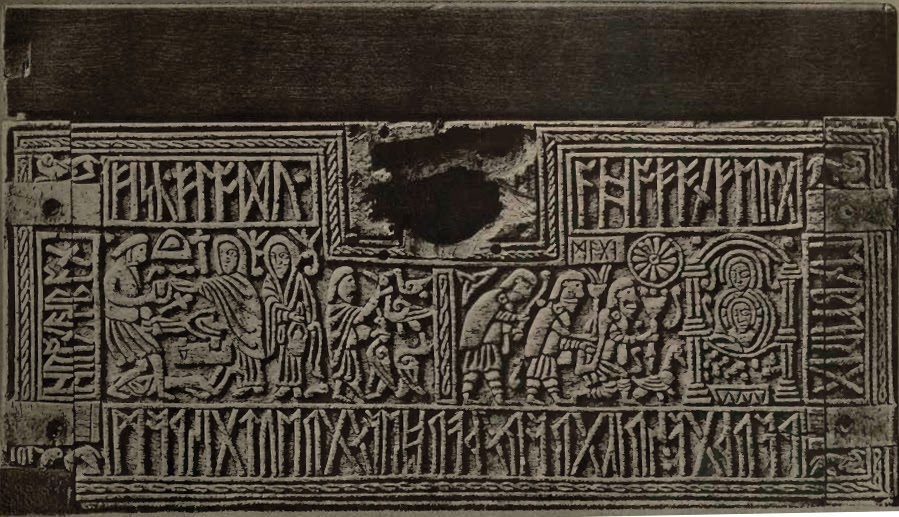
\includegraphics[width=\textwidth]{chapters/img/franks-casket.png}
    \caption{The Franks casket}
    \label{fig:franks-casket}
\end{figure}

\begin{quote}
    \gll fisc~. flodu~. ahof on ferg~|~enberig~| warþ ga:sric grorn\\
    fish flood.\textsc{nom} lifted on mountain  became  rage-beast sad\\\newline
    \gll þær he on greut giswom~| hronæs ban\\
    where he on grit swam whale.\textsc{gen} bone\\\newline
    \trans `The flood lifted a fish onto the cliffs. The angry beast became sad where he swam in the sand. Whalebone.'
\end{quote}



\end{texts}

\begin{texts}{Old Saxon worm charm: \emph{Contra vermes} `Against worms'}
This text is also later, written in the 10th century. It's in Old Saxon,\il{Saxon, Old} the closest first-millennium relative of Old English. See if you can spot alliteration!\is{alliteration} You may also notice the absence of Anglo-Frisian Brightening.\is{Anglo-Frisian Brightening}

\begin{quote}
    \gll Gang út nesso. mid nigun. nessiklinon.\\
    go out worm with nine worm-small-\textsc{dat.pl}\\\newline
    \gll út fana themo. margę.~| an that. ben.\\
    out from the.\textsc{dat} marrow.\textsc{dat}  to the.\textsc{acc} bone.\textsc{acc}\\\newline
    \gll fan themo. bene. an that. flesg\\
    from the.\textsc{dat} bone.\textsc{dat} to the.\textsc{acc} flesh.\textsc{acc}\\\newline
    \gll ut fan themo.~| flesgke. an thia hud.\\
    out from the.\textsc{dat} flesh to the.\textsc{acc} skin.\textsc{acc}\\\newline
    \gll ut fan thera. hud. an thesa strala.\\
    out from the.\textsc{dat} skin.\textsc{dat} to this.\textsc{acc} arrow.\textsc{acc}\\\newline
    \gll drohtin uuerthe so.\\
    lord become.\textsc{sbjv} so\\\newline
    \trans `Get out, worm, with nine little worms! Out from the marrow to the bone, from the bone to the flesh, out from the flesh to the skin, out from the skin to this arrow. Lord, may it be so!'
\end{quote}


\end{texts}

\begin{texts}{The Law of Æþelberht}\is{legal language|(}
King Æþelberht\ia{Æþelberht (King of Kent)} of Kent (/ˈæðelberxt/) lived between 550--616. One of the things he is known for is being one of the very first Old English kings who converted to Christianity.\is{Christianity} Another thing he's known for, more relevant here, is his famous law code, which provides a lot of detail on what sort of fines applied under what circumstances at the time. This code is actually the earliest such work attested in any Germanic language. We give you a few lines below. If you'd like to know what the punishment was for making someone lose their tooth or the ability to speak, read on!\footnote{From the manuscript\is{manuscripts} at \url{https://earlyenglishlaws.ac.uk/laws/manuscripts/h/?tp=s&nb=69}, ff. 2r-2v; accessed May 2020; punctuation kept as in the original. A Present Day English translation as well as a transliteration of the entire work can be found here: \url{https://earlyenglishlaws.ac.uk/laws/texts/abt/}. The line numbering follows this version for ease of comparison, but in the Old English manuscript the different fines start and begin at different points of the individual lines, marked by a red capital letter in the manuscript.\is{manuscripts}}

\begin{quote}
    \gll 31 Gif fri man ƿið fries mannes ƿif ʒeliʒeþ · his ƿerʒelde abicʒe. ⁊ oðer ƿif his aʒenum scætte beʒete · ⁊ ðæm oðrum æt þam ʒebrenʒe·\\
    ~ if free man with free.\textsc{gen} man.\textsc{gen} wife lies ~ his wergild pay-off.\textsc{sbjv} and other wife his own.\textsc{dat} money.\textsc{dat} get.\textsc{sbjv} ~ and the.\textsc{dat} other.\textsc{dat} at that.\textsc{dat} bring.\textsc{sbjv}\\\newline
    \trans `If a free man sleeps with another free man's wife, he should pay his wergild and pay for another wife with his own money and bring her to the other man at home.'
    
    \gll 32 Gif man rihthamscyld þurh stinð. mid ƿeorðe forʒelde·\\
    ~ if man rihthamscyld through pierces with worth.\textsc{dat} pay.\textsc{sbjv}\\\newline
    \trans `If someone pierces the \emph{rihthamscyld},\footnote{The word \textit{hamscyld} is extremely difficult to translate, and scholars have been speculating as to what this might mean exactly. See e.g. \citet{Ammon2002} for some ideas.} let him pay with its worth.'
    
    \gll 33 Gif feaxfanʒ ʒeweorð. l. sceatta to bote·\\
    ~ if hair-grip happens 50 sceattas to restitution\\\newline
    \trans `If there is seizing of hair, 50 sceattas should be paid as restitution.'
    
    \gll 34 Gif banes blice ƿeorðeþ. iii. scillinʒum ʒebete·\\
    ~ if bone.\textsc{gen} exposure happens 3 shillings pay.\textsc{sbjv}\\\newline
    \trans `If a bone is exposed, 3 shillings should be paid.'
    
    \gll 35 Gif banes bite ƿeorð. IIII. scillinʒum ʒebete·\\
    ~ if bone.\textsc{gen} bite happens 4 shillings pay.\textsc{sbjv}\\\newline
    \trans `If a bone is cut, 4 shillings should be paid.'
    
    \gll 36 Gif sio uterre hion ʒebrocen ƿeorðeþ. x. scillinʒum ʒebete·\\
    ~ if the outer hion broken becomes 10 shillings pay.\textsc{sbjv}\\\newline
    \trans `If the outer bone of the head is broken, 10 shillings should be paid.'
    
    \gll 36.1 Gif butu sien. xx. scillinʒum ʒebete·\\
    ~ if both be.\textsc{sbjv} 20 shillings pay.\textsc{sbjv}\\\newline
    \trans `If both are (broken), 20 shillings should be paid.'
    
    \gll 37 Gif eaxle ʒelæmed ƿeorþeð. xxx. scill ʒebete·\\
    ~ if shoulder lamed becomes 30 shillings pay.\textsc{sbjv}\\\newline
    \trans `If a shoulder is lamed, 30 shillings should be paid.'
    
    \gll 38 Gif oþer eare naƿiht ʒehereð. xxv· scill ʒebete·\\
    ~ if either ear nothing hears 25 shillings pay.\textsc{sbjv}\\\newline
    \trans `If either ear loses hearing, 25 shillings should be paid.'
    
    \gll 39 Gif eare of ƿeorð aslaʒen. xii. scill ʒebete·\\
    ~ if ear off becomes cut 12 shillings pay.\textsc{sbjv}\\\newline
    \trans `If an ear is cut off, 12 shillings should be paid.'
    
    \gll 40 Gif eare þirel ƿeorðeþ· iii· scill ʒebete·\\
    ~ if ear pierced becomes 3 shillings pay.\textsc{sbjv}\\\newline
    \trans `If an ear is pierced, 3 shillings should be paid.'
    
    \gll 41 Gif eare sceard ƿeorðeþ· vi· scill ʒebete·\\
    ~ if ear gashed becomes 6 shillings pay.\textsc{sbjv}\\\newline
    \trans `If an ear is gashed, 6 shillings should be paid.'
    
    \gll 42 Gif eaʒe of ƿeorð. l· scillinʒum ʒebete·\\
    ~ if eye off becomes 50 shillings pay.\textsc{sbjv}\\\newline
    \trans `If an eye is cut out, 50 shillings should be paid.'
    
    \gll 43 Gif muð oþþe eaʒe ƿoh ƿeorðeþ· xii· scill ʒebete.\\
    ~ if mouth or eye damaged becomes 12 shillings pay.\textsc{sbjv}\\\newline
    \trans `If the mouth or eye is damaged, 12 shillings should be paid.'
    
    \gll 44 Gif nasu ðyrel ƿeorð· viiii· scillinʒum ʒebete·\\
    ~ if nose pierced becomes 9 shillings pay.\textsc{sbjv}\\\newline
    \trans `If the nose is pierced, 9 shillings should be paid.'
    
    \gll 44.1 Gif hit sio an hleore iii· scill ʒebete.\\
    ~ if it be.\textsc{sbjv} on cheek.\textsc{dat} 3 shillings pay.\textsc{sbjv}\\\newline
    \trans `If it (the piercing) is on the cheek, 3 shillings should be paid.'
    
    \gll 44.2 Gif butu ðyrele sien. vi. scill ʒebete·\\
    ~ if both pierced be.\textsc{sbjv} 6 shillings pay.\textsc{sbjv}\\\newline
    \trans `If both are pierced, 6 shillings should be paid.'
    
    \gll 45 Gif nasu ælcor sceard ƿeorð ʒehwylc· vi· scill ʒebete·\\
    ~ if nose otherwise gashed becomes each 6 shillings pay.\textsc{sbjv}\\\newline
    \trans `If the nose otherwise becomes gashed, 6 shillings should be paid for each.'
    
    \gll 46 Gif ðirel ƿeorþ· vi· scill ʒebete·\\
    ~ if pierced becomes 6 shillings pay.\textsc{sbjv}\\\newline
    \trans `If it becomes pierced, 6 shillings should be paid.'
    
    \gll 47 Se þe cinban forslæhð mid· xx· scillinʒum forʒelde.\\
    ~ he who chin-bone breaks with 20 shillings pay.\textsc{sbjv}\\\newline
    \trans `He who breaks the jawbone should pay 20 shillings.'
    
    \gll 48 Æt þam feoƿer toðum fyrestum æt ʒehƿylcum· vi· scillinʒas.\\
    ~ at the.\textsc{dat} four teeth.\textsc{dat} first.\textsc{dat} at each 6 shillings\\\newline
    \trans `The four front teeth are worth 6 shillings each.'
    
    \gll 48.1 Se toþ se þanne bi standeþ· iiii· sci·\\
    ~ the tooth that then by stands 4 shillings\\\newline
    \trans `The tooth next to them is worth 4 shillings.'
    
    \gll 48.2 Se þe ðonne bi ðam standeþ. iii· scill.\\
    ~ that which then by that.\textsc{dat} stands 3 shillings\\\newline
    \trans `The one next to that one is worth 3 shillings.'
    
    \gll 48.3 And þõn siþþan ʒehƿylc scillinʒ·\\
    ~ and then after each shilling\\\newline
    \trans `And one shilling for each one (tooth) after.'
    
    \gll 49 Gif spræc aƿyrd ƿeorþ. xii· scillinʒas.\\
    ~ if speech damaged becomes 12 shillings\\\newline
    \trans `If speech becomes damaged, 12 shillings should be paid.'\is{legal language|)}
\end{quote}


\end{texts}

\begin{texts}{The Gothic Bible}
This text is from the 4th-century \ili{Gothic} Bible translation. It's an excerpt of the parable of the Sower and the Seed (Mark 4, verses 3--4), like the one we saw in Exercise \ref{sower-and-seed} of \chapref{introduction}. \ili{Gothic} is an East Germanic language, and is often thought to be the closest Germanic language to \ili{Proto-Germanic} because of its early attestation and complex morphology.

\begin{quote}
    \gll hauseiþ! Sai, urrann sa saiands du saian fraiwa seinamma.\\
    hear.\textsc{2pl.imp} see out.ran the sower.\textsc{nom} to sow seed.\textsc{dat} his.\textsc{dat}\\\newline
    \gll Jah warþ, miþþanei saiso, sum raihtis gadraus faur wig,\\
    and became while sowed some though fell to way\\\newline
    \gll jah qemun fuglos jah fretun þata.\\
    and came.\textsc{3pl} bird.\textsc{nom.pl} and ate that.\textsc{acc}\\\newline
    \trans `Listen! The sower went out to sow his seed. And it happened that, while he sowed, some fell onto the road, and birds\is{birds} came and ate it.'
\end{quote}


\end{texts}

\begin{texts}{The Golden Horn of Gallehus}
Another runic\is{runes} inscription, this time in something close to Proto-\ili{Norse}, the ancestor language of the North Germanic branch. This one was found on a drinking horn made of sheet gold, one of a pair, in Gallehus, Denmark. It dates to the early 5th century CE. Discovered in 1734, the horn was stolen and melted down in 1802. Fortunately, detailed drawings had been made, so that a replica could be constructed, and the ancient inscription itself was not lost.


\begin{figure}[H]
        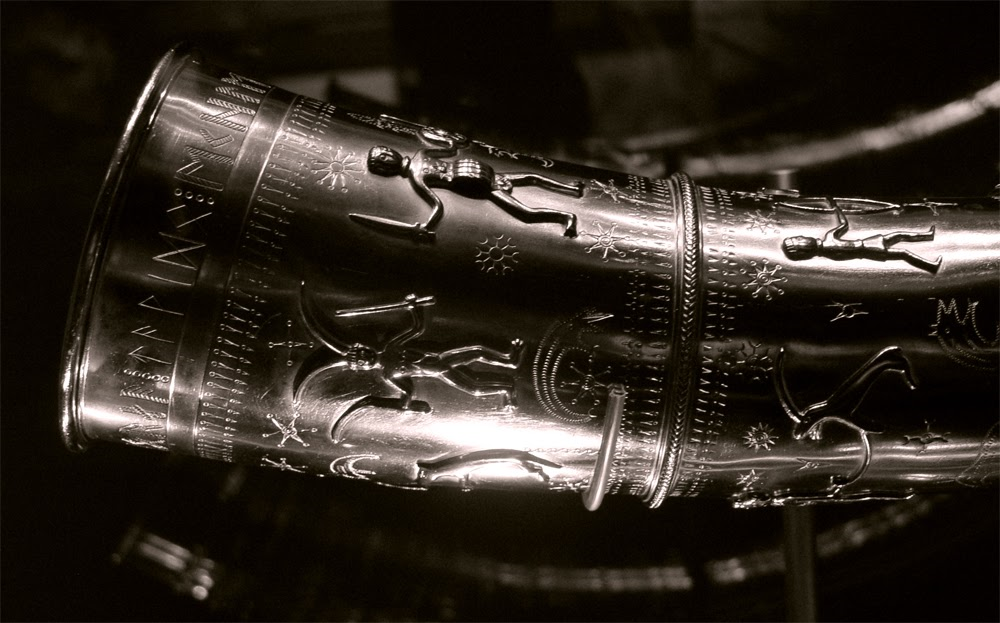
\includegraphics[height=0.2\textheight]{chapters/img/horn_of_gallehus.png}
    \caption{The Golden Horn of Gallehus replica (Photo by Bloodofox, licensed under CC-BY-SA 3.0)}
    \label{fig:horn-of-hallehus}
\end{figure}


\noindent The inscription is in the Older Futhark, and consists of a single clause. The verb in this clause is a characteristically Germanic weak past tense\is{weak verbs} form!


\begin{quote}
    \textarc{ekhlewagastiR{\doubledot}holtijaR{\doubledot}horna{\doubledot}tawido{\doubledot}}\\
    \gll ek hlewagastiz: holtijaz: horna: tawido:\\
    I Hlewagastiz Holtijaz horn made\\\newline
    \trans `I, Hlewagastiz Holtijaz,\ia{Holtijaz, Hlewagastiz} made this horn.'\is{runes}
\end{quote}

\end{texts}
\begin{furtherreading}
If you're interested in the history and archaeology\is{archaeology} of Britain, \citet{Fleming2010} is a recent and masterful overview, starting before the \emph{aduentus Saxonum}\is{\emph{aduentus Saxonum}} and covering the whole period up to 1070 CE. For Indo-European history and archaeology, \citet{Anthony2007} should be the first place to look.\is{archaeology}

\citet{Robinson1992} is a great introduction to the early Germanic languages, and \citet{Clackson2007} introduces comparative Indo-European linguistics. On the general methodology of historical linguistics and linguistic reconstruction,\is{reconstruction} there are many good textbooks available: we'd recommend \citet{Campbell2013}.

\citet{Findell2014} is a handy guide to the world of Germanic and Old English runes.\is{runes} There is a substantial literature on Germanic and Old English alliterative\is{alliteration} verse, but from a linguistic perspective the clearest overview is to be found in \citet{McCullyHilles2005}. Finally, if you'd like to find out more about the specific phonological, morphological and syntactic changes that characterized the prehistory of English, the first two volumes of Ringe's \emph{Linguistic History of English} (\citealp{Ringe2017}; \citealp{RingeTaylor2014}) are treasure troves of information, as is \citet{Fulk2018} -- though be warned that they are not exactly light bedtime reading.
\end{furtherreading}
